% Options for packages loaded elsewhere
\PassOptionsToPackage{unicode}{hyperref}
\PassOptionsToPackage{hyphens}{url}
\documentclass[
]{book}
\usepackage{xcolor}
\usepackage{amsmath,amssymb}
\setcounter{secnumdepth}{5}
\usepackage{iftex}
\ifPDFTeX
  \usepackage[T1]{fontenc}
  \usepackage[utf8]{inputenc}
  \usepackage{textcomp} % provide euro and other symbols
\else % if luatex or xetex
  \usepackage{unicode-math} % this also loads fontspec
  \defaultfontfeatures{Scale=MatchLowercase}
  \defaultfontfeatures[\rmfamily]{Ligatures=TeX,Scale=1}
\fi
\usepackage{lmodern}
\ifPDFTeX\else
  % xetex/luatex font selection
\fi
% Use upquote if available, for straight quotes in verbatim environments
\IfFileExists{upquote.sty}{\usepackage{upquote}}{}
\IfFileExists{microtype.sty}{% use microtype if available
  \usepackage[]{microtype}
  \UseMicrotypeSet[protrusion]{basicmath} % disable protrusion for tt fonts
}{}
\makeatletter
\@ifundefined{KOMAClassName}{% if non-KOMA class
  \IfFileExists{parskip.sty}{%
    \usepackage{parskip}
  }{% else
    \setlength{\parindent}{0pt}
    \setlength{\parskip}{6pt plus 2pt minus 1pt}}
}{% if KOMA class
  \KOMAoptions{parskip=half}}
\makeatother
\usepackage{color}
\usepackage{fancyvrb}
\newcommand{\VerbBar}{|}
\newcommand{\VERB}{\Verb[commandchars=\\\{\}]}
\DefineVerbatimEnvironment{Highlighting}{Verbatim}{commandchars=\\\{\}}
% Add ',fontsize=\small' for more characters per line
\usepackage{framed}
\definecolor{shadecolor}{RGB}{248,248,248}
\newenvironment{Shaded}{\begin{snugshade}}{\end{snugshade}}
\newcommand{\AlertTok}[1]{\textcolor[rgb]{0.94,0.16,0.16}{#1}}
\newcommand{\AnnotationTok}[1]{\textcolor[rgb]{0.56,0.35,0.01}{\textbf{\textit{#1}}}}
\newcommand{\AttributeTok}[1]{\textcolor[rgb]{0.13,0.29,0.53}{#1}}
\newcommand{\BaseNTok}[1]{\textcolor[rgb]{0.00,0.00,0.81}{#1}}
\newcommand{\BuiltInTok}[1]{#1}
\newcommand{\CharTok}[1]{\textcolor[rgb]{0.31,0.60,0.02}{#1}}
\newcommand{\CommentTok}[1]{\textcolor[rgb]{0.56,0.35,0.01}{\textit{#1}}}
\newcommand{\CommentVarTok}[1]{\textcolor[rgb]{0.56,0.35,0.01}{\textbf{\textit{#1}}}}
\newcommand{\ConstantTok}[1]{\textcolor[rgb]{0.56,0.35,0.01}{#1}}
\newcommand{\ControlFlowTok}[1]{\textcolor[rgb]{0.13,0.29,0.53}{\textbf{#1}}}
\newcommand{\DataTypeTok}[1]{\textcolor[rgb]{0.13,0.29,0.53}{#1}}
\newcommand{\DecValTok}[1]{\textcolor[rgb]{0.00,0.00,0.81}{#1}}
\newcommand{\DocumentationTok}[1]{\textcolor[rgb]{0.56,0.35,0.01}{\textbf{\textit{#1}}}}
\newcommand{\ErrorTok}[1]{\textcolor[rgb]{0.64,0.00,0.00}{\textbf{#1}}}
\newcommand{\ExtensionTok}[1]{#1}
\newcommand{\FloatTok}[1]{\textcolor[rgb]{0.00,0.00,0.81}{#1}}
\newcommand{\FunctionTok}[1]{\textcolor[rgb]{0.13,0.29,0.53}{\textbf{#1}}}
\newcommand{\ImportTok}[1]{#1}
\newcommand{\InformationTok}[1]{\textcolor[rgb]{0.56,0.35,0.01}{\textbf{\textit{#1}}}}
\newcommand{\KeywordTok}[1]{\textcolor[rgb]{0.13,0.29,0.53}{\textbf{#1}}}
\newcommand{\NormalTok}[1]{#1}
\newcommand{\OperatorTok}[1]{\textcolor[rgb]{0.81,0.36,0.00}{\textbf{#1}}}
\newcommand{\OtherTok}[1]{\textcolor[rgb]{0.56,0.35,0.01}{#1}}
\newcommand{\PreprocessorTok}[1]{\textcolor[rgb]{0.56,0.35,0.01}{\textit{#1}}}
\newcommand{\RegionMarkerTok}[1]{#1}
\newcommand{\SpecialCharTok}[1]{\textcolor[rgb]{0.81,0.36,0.00}{\textbf{#1}}}
\newcommand{\SpecialStringTok}[1]{\textcolor[rgb]{0.31,0.60,0.02}{#1}}
\newcommand{\StringTok}[1]{\textcolor[rgb]{0.31,0.60,0.02}{#1}}
\newcommand{\VariableTok}[1]{\textcolor[rgb]{0.00,0.00,0.00}{#1}}
\newcommand{\VerbatimStringTok}[1]{\textcolor[rgb]{0.31,0.60,0.02}{#1}}
\newcommand{\WarningTok}[1]{\textcolor[rgb]{0.56,0.35,0.01}{\textbf{\textit{#1}}}}
\usepackage{longtable,booktabs,array}
\usepackage{calc} % for calculating minipage widths
% Correct order of tables after \paragraph or \subparagraph
\usepackage{etoolbox}
\makeatletter
\patchcmd\longtable{\par}{\if@noskipsec\mbox{}\fi\par}{}{}
\makeatother
% Allow footnotes in longtable head/foot
\IfFileExists{footnotehyper.sty}{\usepackage{footnotehyper}}{\usepackage{footnote}}
\makesavenoteenv{longtable}
\usepackage{graphicx}
\makeatletter
\newsavebox\pandoc@box
\newcommand*\pandocbounded[1]{% scales image to fit in text height/width
  \sbox\pandoc@box{#1}%
  \Gscale@div\@tempa{\textheight}{\dimexpr\ht\pandoc@box+\dp\pandoc@box\relax}%
  \Gscale@div\@tempb{\linewidth}{\wd\pandoc@box}%
  \ifdim\@tempb\p@<\@tempa\p@\let\@tempa\@tempb\fi% select the smaller of both
  \ifdim\@tempa\p@<\p@\scalebox{\@tempa}{\usebox\pandoc@box}%
  \else\usebox{\pandoc@box}%
  \fi%
}
% Set default figure placement to htbp
\def\fps@figure{htbp}
\makeatother
\setlength{\emergencystretch}{3em} % prevent overfull lines
\providecommand{\tightlist}{%
  \setlength{\itemsep}{0pt}\setlength{\parskip}{0pt}}
\usepackage[]{natbib}
\bibliographystyle{plainnat}
\usepackage{booktabs}
\usepackage{bookmark}
\IfFileExists{xurl.sty}{\usepackage{xurl}}{} % add URL line breaks if available
\urlstyle{same}
\hypersetup{
  pdftitle={Creating and Labeling Data},
  pdfauthor={Samuel Rowe adapted from Mitchell (2020)},
  hidelinks,
  pdfcreator={LaTeX via pandoc}}

\title{Creating and Labeling Data}
\author{Samuel Rowe adapted from Mitchell (2020)}
\date{2026-08-30}

\begin{document}
\maketitle

{
\setcounter{tocdepth}{1}
\tableofcontents
}
\begin{Shaded}
\begin{Highlighting}[]
\NormalTok{bookdown}\SpecialCharTok{::}\FunctionTok{render\_book}\NormalTok{()}
\end{Highlighting}
\end{Shaded}

\chapter*{Overview}\label{overview}
\addcontentsline{toc}{chapter}{Overview}

Topics:

\begin{enumerate}
\def\labelenumi{\arabic{enumi}.}
\tightlist
\item
  Creating Data
\item
  Labeling Data
\item
  Exercises
\end{enumerate}

\chapter{Creating Data}\label{creating-data}

The \emph{generate} and replace will be the workhorses of creating and modifying variables
We'll deal with generating binary variables. We'll look into missing data and how to handle it. \emph{Note: Please do not label your missing data, it just is a pain to deal with later}
The \emph{egen} command is also a very practical and useful (I wish other software
packages had this type of command). We'll deal with strings and converting between numerics and strings.

\section{Creating and changing variables}\label{creating-and-changing-variables}

One of the most basic tasks is to create, replace, and modify variables. Stata provides some nice and easy commands to work with variable generation and modification relative to other statistical software packages: \emph{generate} and \emph{replace}. These will be the workhorses for the creation and modification of variables.

As we go through Mitchell's Chapter 6, we'll see that these are not the only two commands we will utilize. For example, Stata has a very helpful command called \emph{egen}. It can be used to create new variables from old variables, especially when working with groups of observations. \emph{Egen} becomes even more helpful when it is combined with \emph{bysort}. We can sort our group and find the max, min, sum, etc. of a group of observations, which can come in handy when we are working with panel data. Furthermore, using indexes can make our generation commands more useful for creating lags or rebasing our data.

\subsection{Generate command}\label{generate-command}

The \emph{generate} or \emph{gen} command is one command that you may already have plenty of experience with, but there are some helpful tips when working with generate. What we'll do first is to create a new variable called potential experience and potential experience squared.

Let's look at ages for workers earning weekly wages.

\begin{Shaded}
\begin{Highlighting}[]
\NormalTok{cd }\StringTok{"/Users/Sam/Desktop/Data/CPS"}
\KeywordTok{use}\NormalTok{ smalljul25pub, }\KeywordTok{clear}
\KeywordTok{summarize}\NormalTok{ prtage }\KeywordTok{if}\NormalTok{ prerelg==1}
\KeywordTok{generate}\NormalTok{ pot\_exp=prtage{-}16}
\KeywordTok{summarize}\NormalTok{ pot\_exp }\KeywordTok{if}\NormalTok{ prerelg==1}
\end{Highlighting}
\end{Shaded}

\begin{verbatim}
/Users/Sam/Desktop/Data/CPS

    Variable |        Obs        Mean    Std. dev.       Min        Max
-------------+---------------------------------------------------------
      prtage |      9,635    42.43778    14.74111         15         85

(28,617 missing values generated)

    Variable |        Obs        Mean    Std. dev.       Min        Max
-------------+---------------------------------------------------------
     pot_exp |      9,635    26.43778    14.74111         -1         69
\end{verbatim}

Look for outliers and generate a histogram for outliers

\begin{Shaded}
\begin{Highlighting}[]
\KeywordTok{histogram}\NormalTok{ pot\_exp }\KeywordTok{if}\NormalTok{ prerelg==1}
\KeywordTok{graph} \KeywordTok{export} \StringTok{"jul\_25\_pot\_exp.png"}\NormalTok{, }\KeywordTok{replace}
\end{Highlighting}
\end{Shaded}

\begin{figure}
\centering
\pandocbounded{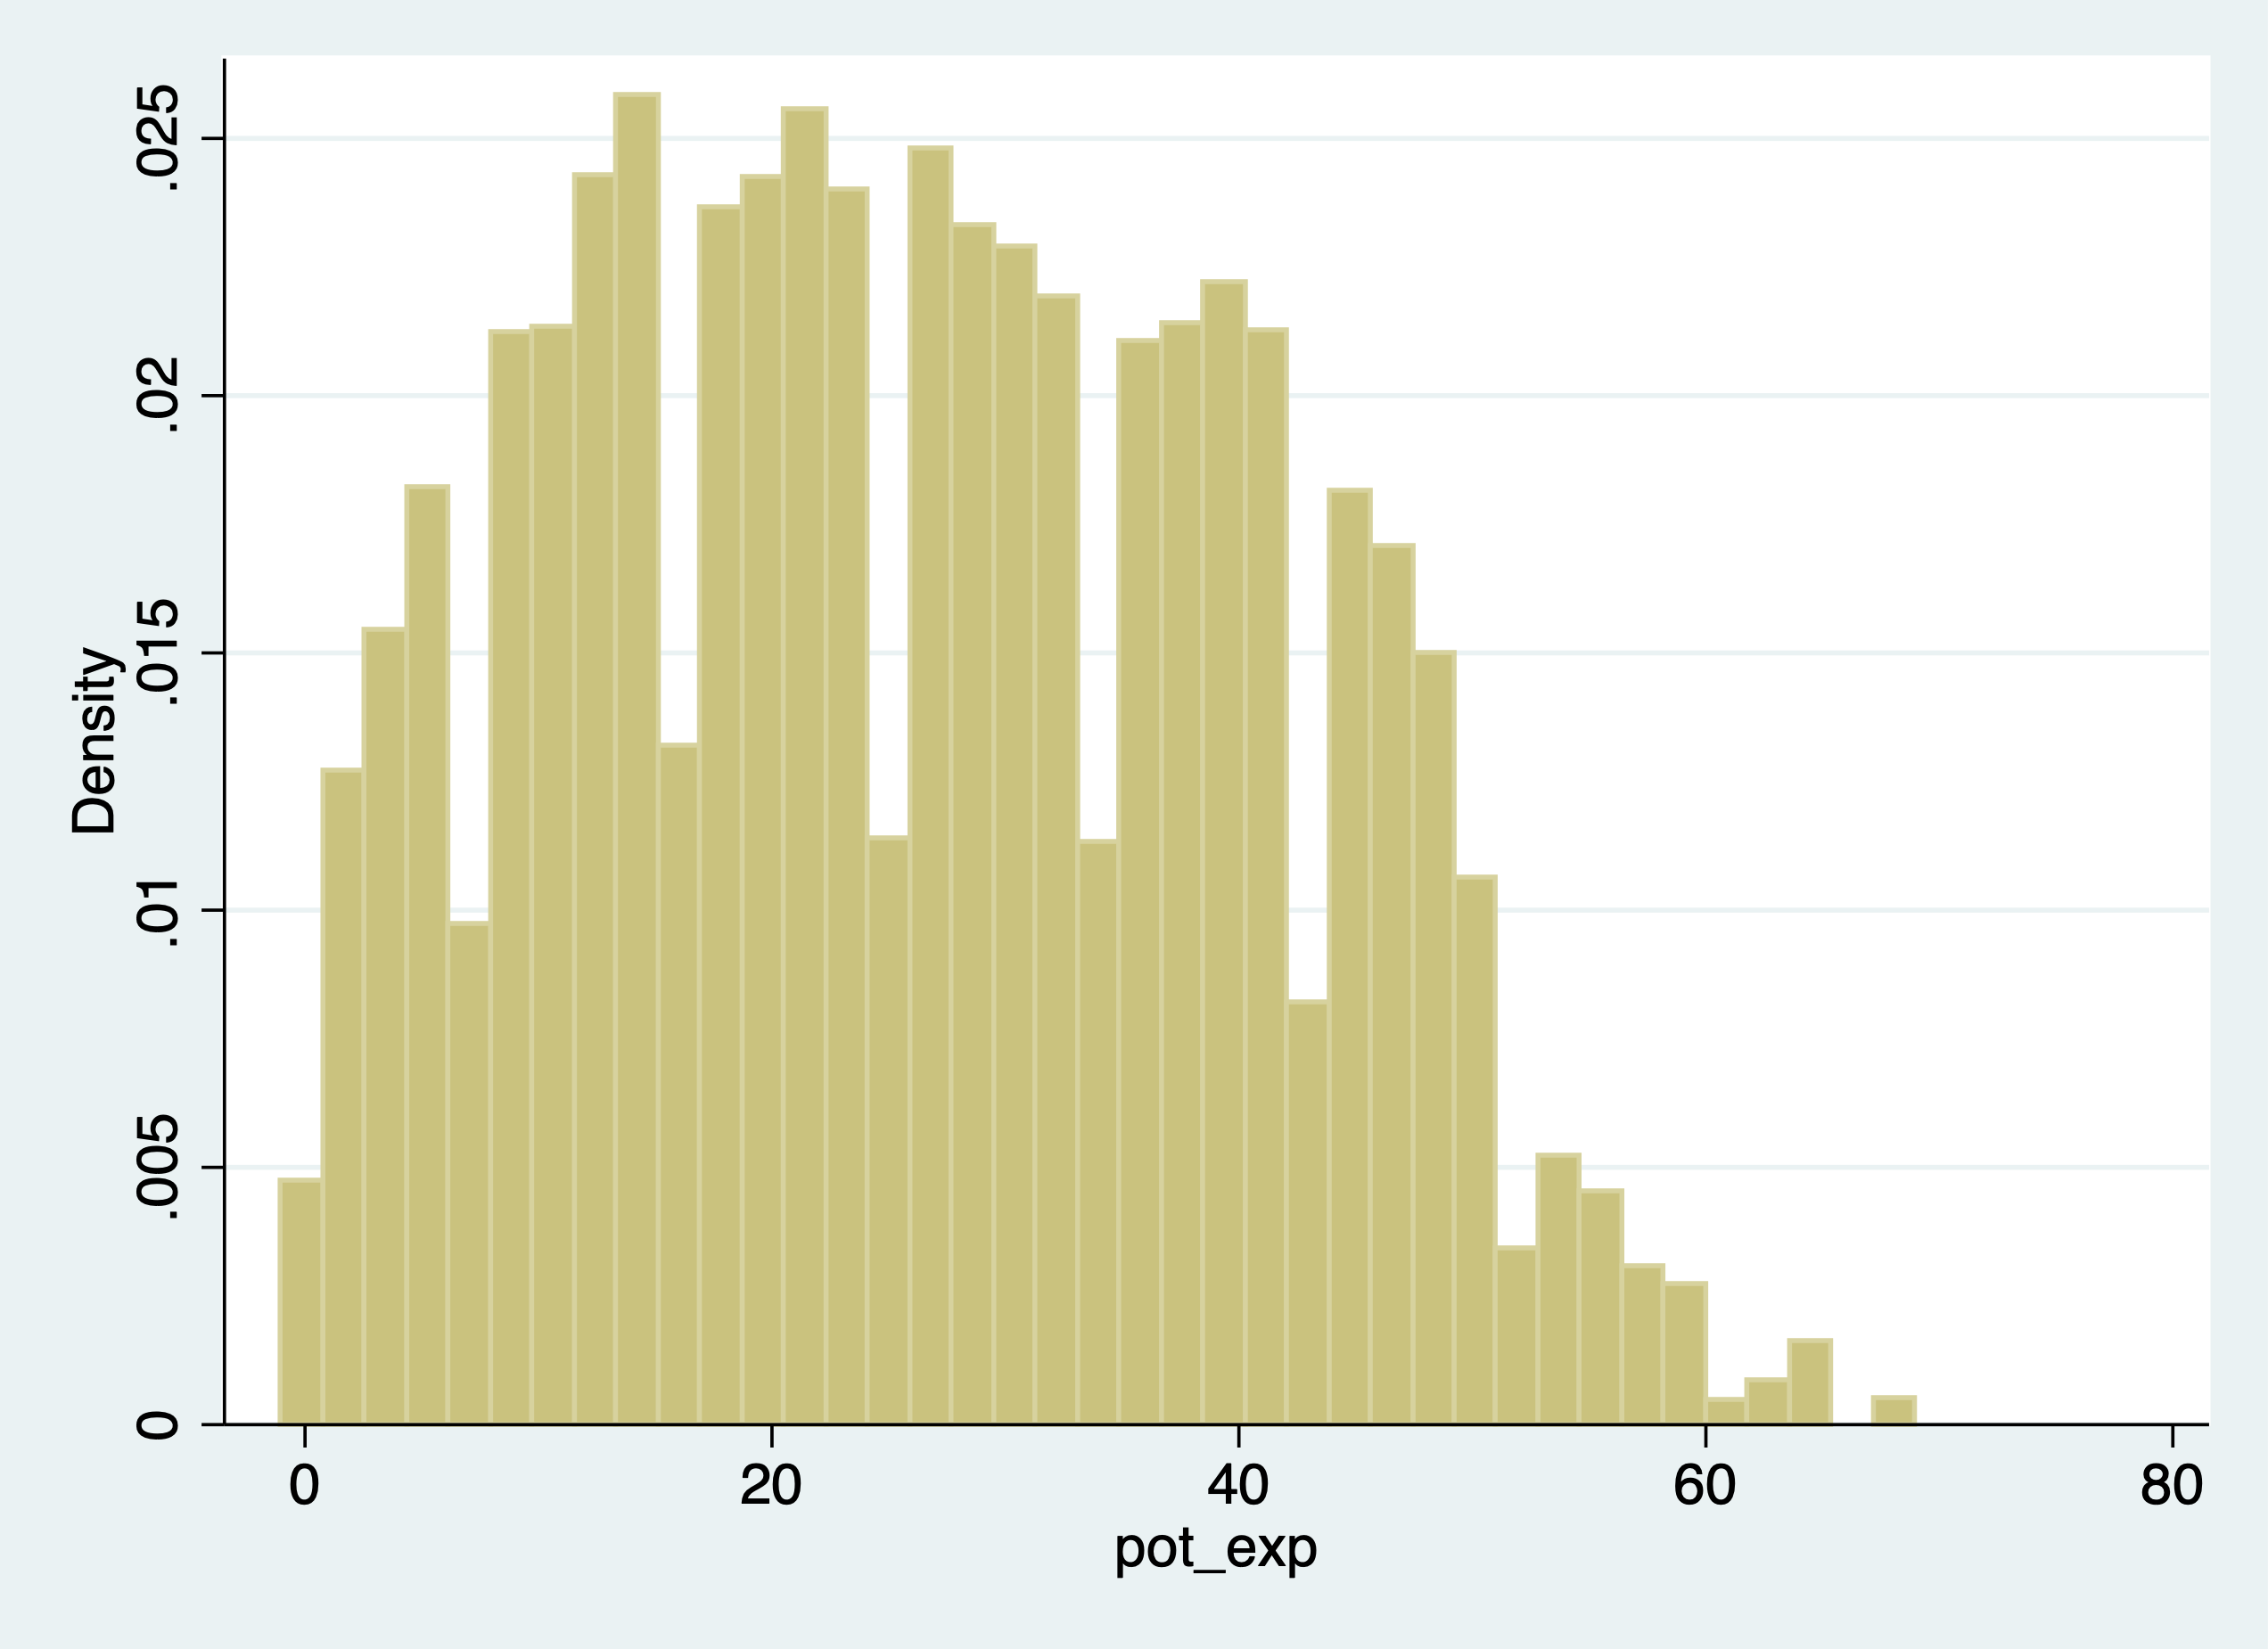
\includegraphics[keepaspectratio,alt={Potential Experience}]{jul_25_pot_exp.png}}
\caption{Potential Experience}
\end{figure}

Now let's create a new variable for potential experience squared. We have two options:

\begin{Shaded}
\begin{Highlighting}[]
\KeywordTok{gen}\NormalTok{ pot\_exp2 = pot\_exp*pot\_exp}
\KeywordTok{sum}\NormalTok{ pot\_exp2}
\KeywordTok{drop}\NormalTok{ pot\_exp2}

\KeywordTok{gen}\NormalTok{ pot\_exp2 = pot\_exp\^{}2}
\KeywordTok{sum}\NormalTok{ pot\_exp2}
\end{Highlighting}
\end{Shaded}

\begin{verbatim}
(28,617 missing values generated)

    Variable |        Obs        Mean    Std. dev.       Min        Max
-------------+---------------------------------------------------------
    pot_exp2 |     93,635    1269.006    1345.314          0       4761


(28,617 missing values generated)

    Variable |        Obs        Mean    Std. dev.       Min        Max
-------------+---------------------------------------------------------
    pot_exp2 |     93,635    1269.006    1345.314          0       4761
\end{verbatim}

\textbf{Notice!} Our age variable, prtage, is missing when the value is -1. The data dictionary provides us the information that -1 is a holder for missing data. Please note that when missing values are ``.'', we will see missings in an outlier check! Why? Because missing values are considered \textbf{very large values}. This is important because when creating binary or categorical variables through qualifiers, make sure you top code your qualifiers.

For example, if we are creating a binary on part-time vs full-time. We need to top code so we don't count missing hours as full-time workers,

\begin{Shaded}
\begin{Highlighting}[]
\KeywordTok{gen}\NormalTok{ fulltime }\KeywordTok{if}\NormalTok{ hours \textgreater{} 35 \& hours \textless{} 999999,}
\end{Highlighting}
\end{Shaded}

Alternatively, you can use the missing function.

\begin{Shaded}
\begin{Highlighting}[]
\KeywordTok{gen}\NormalTok{ fulltime }\KeywordTok{if}\NormalTok{ hours \textgreater{} 35 \& !}\FunctionTok{missing}\NormalTok{(hours)}
\end{Highlighting}
\end{Shaded}

Let's generate weekly earnings and plot the data. The CPS data dictionary tells us that pternwa is the weekly earnings, but it needs to be divided by 100 to get two decimal places.

\begin{Shaded}
\begin{Highlighting}[]
\KeywordTok{gen}\NormalTok{ earnings=pternwa/100}
\KeywordTok{histogram}\NormalTok{ earnings }\KeywordTok{if}\NormalTok{ prerelg==1, }\BaseNTok{title}\NormalTok{(Weekly Earnings)}
\KeywordTok{graph} \KeywordTok{export} \StringTok{"jul\_25\_weekly\_earnings.png"}\NormalTok{, }\KeywordTok{replace}
\end{Highlighting}
\end{Shaded}

\begin{figure}
\centering
\pandocbounded{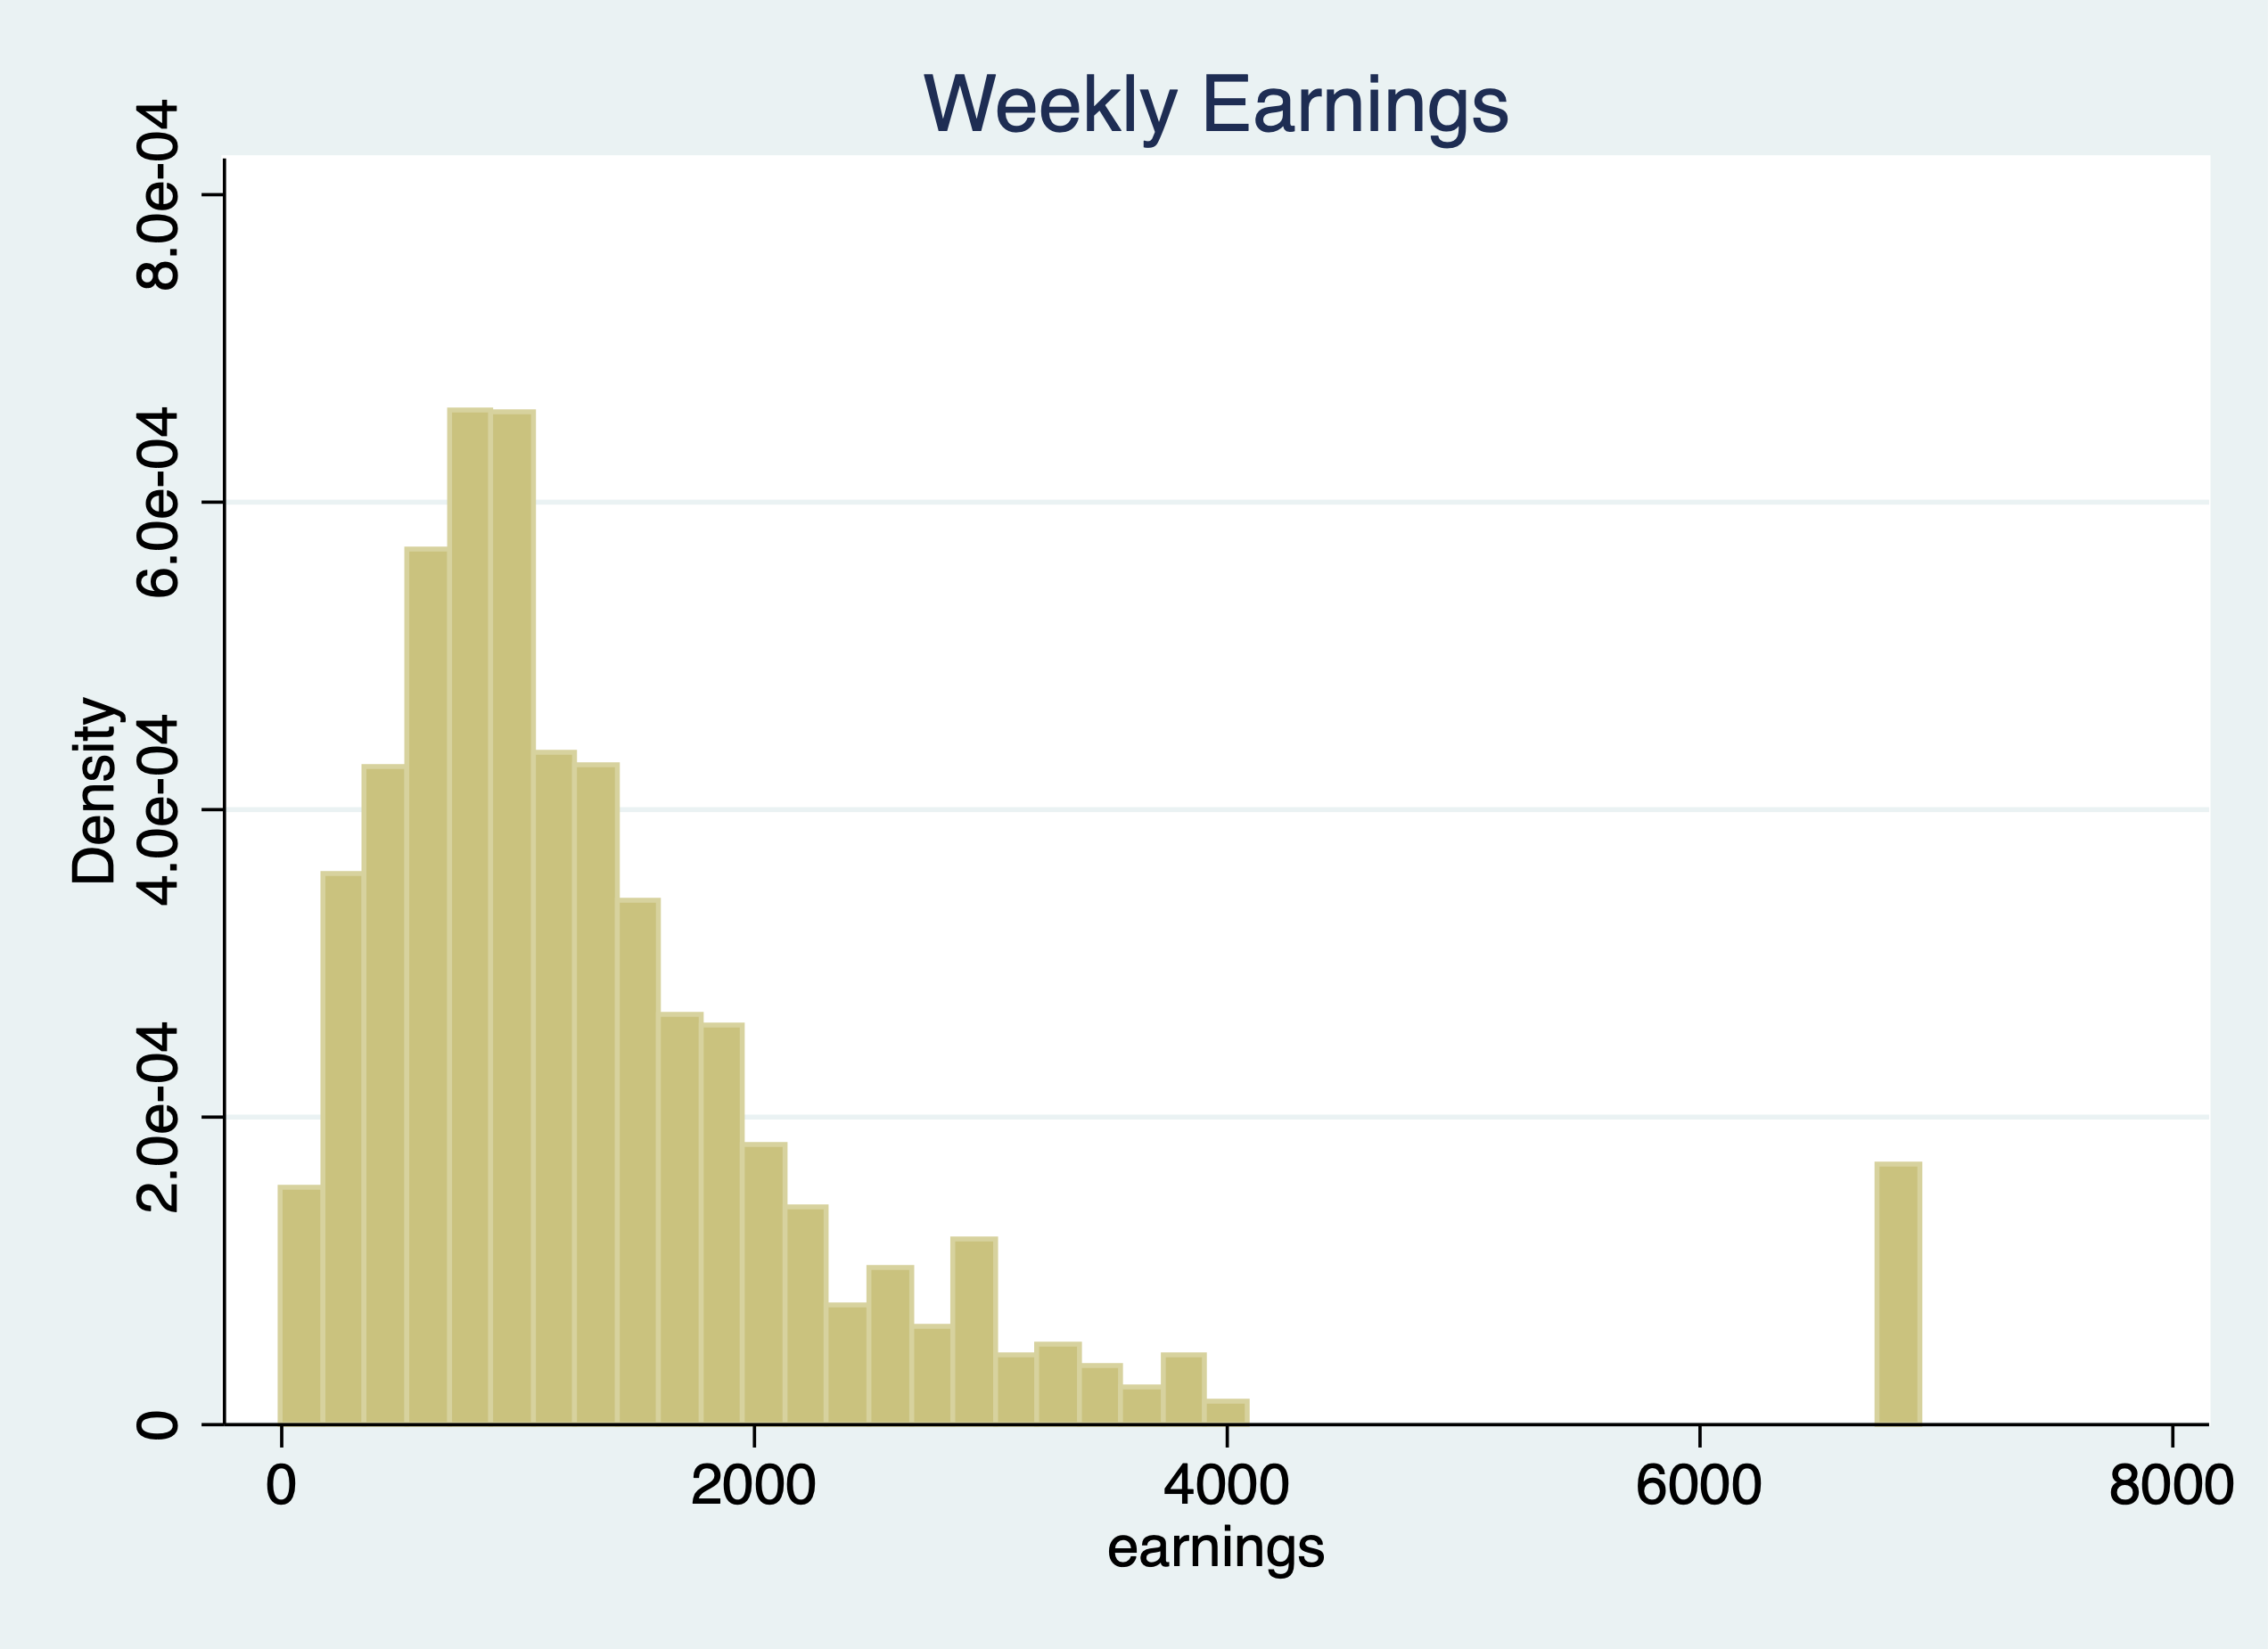
\includegraphics[keepaspectratio,alt={Weekly Earnings}]{jul_25_weekly_earnings.png}}
\caption{Weekly Earnings}
\end{figure}

Another helpful trick is the before and after options. It might be helpful to have the newly created variable next to a similar variable, so let's drop our variable and generate it again with the after option

\begin{Shaded}
\begin{Highlighting}[]
\KeywordTok{drop}\NormalTok{ weekwage}
\KeywordTok{gen}\NormalTok{ hrlyearn = pternwa/pehract1, after(pternwa)}
\KeywordTok{drop}\NormalTok{ hrlyearn}
\KeywordTok{gen}\NormalTok{ hrlyearn = pternwa/pehract1, before(pternwa)}
\end{Highlighting}
\end{Shaded}

\subsection{Replace}\label{replace}

We use our \emph{replace} command to modify a variable that has already been created. Similar to generate, you probably already have experience with replace, but we'll go over some useful tips.

Qualifiers will be an essential part of your syntax when using the \emph{replace} command.

Let's generate a variable called marital status and look at married and nevermarried variables.

\begin{Shaded}
\begin{Highlighting}[]
\KeywordTok{quietly}\NormalTok{ cd }\StringTok{"/Users/Sam/Desktop/Econ 645/Data/Mitchell"}
\KeywordTok{quietly} \KeywordTok{use}\NormalTok{ wws, }\KeywordTok{clear}
\KeywordTok{tabulate}\NormalTok{ married nevermarried}
\end{Highlighting}
\end{Shaded}

\begin{verbatim}
           |   Woman never been
           |        married
   married |         0          1 |     Total
-----------+----------------------+----------
         0 |       570        234 |       804 
         1 |     1,440          2 |     1,442 
-----------+----------------------+----------
     Total |     2,010        236 |     2,246 
\end{verbatim}

We'll generate a new variable called maritalstatus.

\begin{Shaded}
\begin{Highlighting}[]
\KeywordTok{gen}\NormalTok{ maritalstatus = .}
\end{Highlighting}
\end{Shaded}

I recommend generating a new categorical variable as missing instead of zero, because this prevents missing variables from being categorized as 0 when applicable.

We generally use qualifiers ``=, \textgreater, \textless, \textgreater=, \textless=, !'' when working with replace. Let's replace the marital status variable with married and nevermarried as qualifiers

\begin{Shaded}
\begin{Highlighting}[]
\KeywordTok{replace}\NormalTok{ maritalstatus = 1 }\KeywordTok{if}\NormalTok{ married==0 \& nevermarried==1}
\KeywordTok{replace}\NormalTok{ maritalstatus = 2 }\KeywordTok{if}\NormalTok{ married==1 \& nevermarried==0}
\KeywordTok{replace}\NormalTok{ maritalstatus = 3 }\KeywordTok{if}\NormalTok{ married==0 \& nevermarried==0}
\end{Highlighting}
\end{Shaded}

It's always a good idea to double check the variables against the variables they were created from to make sure your categories are what they are supposed to be.

\begin{Shaded}
\begin{Highlighting}[]
\KeywordTok{tabulate}\NormalTok{ maritalstatus}
\KeywordTok{table}\NormalTok{ maritalstatus married nevermarried}
\end{Highlighting}
\end{Shaded}

\begin{verbatim}
maritalstat |
         us |      Freq.     Percent        Cum.
------------+-----------------------------------
          1 |        234       10.43       10.43
          2 |      1,440       64.17       74.60
          3 |        570       25.40      100.00
------------+-----------------------------------
      Total |      2,244      100.00


---------------------------------------------
              |    Woman never been married  
              |         0        1      Total
--------------+------------------------------
maritalstatus |                              
  1           |                              
    married   |                              
      0       |                234        234
      Total   |                234        234
  2           |                              
    married   |                              
      1       |     1,440               1,440
      Total   |     1,440               1,440
  3           |                              
    married   |                              
      0       |       570                 570
      Total   |       570                 570
  Total       |                              
    married   |                              
      0       |       570      234        804
      1       |     1,440               1,440
      Total   |     2,010      234      2,244
---------------------------------------------
\end{verbatim}

What will be helpful is to label our values, but we'll cover this next week.

We can also use the \emph{replace} command with a continuous variable in the qualifier

Let's create a new variable called over40hours which will be categorized as 1 if it is over 40 hours, and 0 if it is 40 or under.

\begin{Shaded}
\begin{Highlighting}[]
\KeywordTok{generate}\NormalTok{ over40hours = .}
\KeywordTok{replace}\NormalTok{ over40hours = 0 }\KeywordTok{if}\NormalTok{ hours \textless{}= 40}
\end{Highlighting}
\end{Shaded}

We need to make sure we don't include missing values so we need an additional qualifier besides hours \textgreater{} 40. We need to add !missing(hours).

\begin{Shaded}
\begin{Highlighting}[]
\KeywordTok{replace}\NormalTok{ over40hours = 1 }\KeywordTok{if}\NormalTok{ hours \textgreater{} 40 \& !}\FunctionTok{missing}\NormalTok{(hours)}
\end{Highlighting}
\end{Shaded}

Now let's see the results.

\begin{Shaded}
\begin{Highlighting}[]
\KeywordTok{tab}\NormalTok{ over40hours}
\KeywordTok{tab}\NormalTok{ over40hours, }\KeywordTok{sum}\NormalTok{(hours)}
\end{Highlighting}
\end{Shaded}

\begin{verbatim}
over40hours |      Freq.     Percent        Cum.
------------+-----------------------------------
          0 |      1,852       82.60       82.60
          1 |        390       17.40      100.00
------------+-----------------------------------
      Total |      2,242      100.00

            |    Summary of usual hours worked
over40hours |        Mean   Std. dev.       Freq.
------------+------------------------------------
          0 |    34.50054   9.0449086       1,852
          1 |   50.123077   6.6961395         390
------------+------------------------------------
      Total |   37.218109   10.509135       2,242
\end{verbatim}

\section{Numeric expressions and functions}\label{numeric-expressions-and-functions}

Our standard numeric expressions
1. addition +,
2. subtraction -,
3. multiplication *,
4. division /,
5. exponentiation \^{}, and
6. parentheses () for changing order of operation.

We also have some very useful numeric functions built into Stata:

The \emph{int()} function removes any decimals.

The \emph{round()} function rounds a number to the desired decimal place.Please note that this is different from Excel!!!

The \emph{round(x,y)} rounds the numbers to the specified nearest value. Where x is your numeric and y is the nearest value you wish to round to.

For example:
1. if y = 1, round(-5.2,1)=-5 and round(4.5)=5
2. if y=.1, round(10.16,.1)=10.2 and round(34.1345,.1)=34.1
3. if y=10, round(313.34,10)=310 and round(4.52,10)=0

\textbf{Note:} if y is missing, then it will round to the nearest integer round(10.16)=10

The \emph{ln()} function is our natural log function which we use a lot for transforming variables for elasticity estimates.

The \emph{log10()} function is our logarithm base-10 function.

The \emph{sqrt()} function is our square root function

\begin{Shaded}
\begin{Highlighting}[]
    \KeywordTok{display} \KeywordTok{int}\NormalTok{(10.65)}
    \KeywordTok{display} \FunctionTok{round}\NormalTok{(10.65,1)}
    \KeywordTok{display} \FunctionTok{ln}\NormalTok{(10.65)}
    \KeywordTok{display} \FunctionTok{log10}\NormalTok{(10.65)}
    \KeywordTok{display} \FunctionTok{sqrt}\NormalTok{(10.65)}
\end{Highlighting}
\end{Shaded}

\begin{verbatim}
10

11

2.3655599

1.0273496

3.2634338
\end{verbatim}

Please note int(10.65) returns 10, while round(10.65,1) returns 11.

\subsection{Random Numbers and setting seeds}\label{random-numbers-and-setting-seeds}

There are several random number generating functions in Stata.

\emph{runiform()} is a random uniform distribution number generator has a distribution between 0 and 1.

\emph{rnormal(m,sd)} is a random normal distribution number generator without arguments it will assume mean = 0 and sd = 1.

\emph{rchi2(df)} is a random chi-squared distribution number generator where df is the degrees of freedom that need to be specified

Let's look at some examples.

Setting seeds is important if you want someone to replicate your results, since a set seed will generate the same random number each time it is run.

\begin{Shaded}
\begin{Highlighting}[]
\NormalTok{*Set our }\DecValTok{seed}
\KeywordTok{set} \DecValTok{seed}\NormalTok{ 12345}

\NormalTok{*Random uniform distribution }
\KeywordTok{gen}\NormalTok{ runiformtest = runiform()}
\KeywordTok{summarize}\NormalTok{ runiformtest}

\NormalTok{*Random }\FunctionTok{normal}\NormalTok{ distribution}
\KeywordTok{gen}\NormalTok{ rnormaltest = rnormal()}
\KeywordTok{gen}\NormalTok{ rnormaltest2 = rnormal(100,15)}
\KeywordTok{summarize}\NormalTok{ rnormaltest rnormaltest2}

\NormalTok{*Random chi{-}squared distribution}
\KeywordTok{gen}\NormalTok{ rchi2test = rchi2(5)}
\KeywordTok{summarize}\NormalTok{ rchi2test}
\end{Highlighting}
\end{Shaded}

\begin{verbatim}
    Variable |        Obs        Mean    Std. dev.       Min        Max
-------------+---------------------------------------------------------
runiformtest |      2,246    .4924636    .2875376   .0007583   .9985868

    Variable |        Obs        Mean    Std. dev.       Min        Max
-------------+---------------------------------------------------------
 rnormaltest |      2,246     .018436    .9857847  -3.389102   3.372524
rnormaltest2 |      2,246    99.70718    14.77732   47.81652   154.2297

    Variable |        Obs        Mean    Std. dev.       Min        Max
-------------+---------------------------------------------------------
   rchi2test |      2,246    5.063639    3.322998   .1102785    29.2429
\end{verbatim}

\section{Strings}\label{strings}

Working with string can be a pain, but there are some very helpful functions that will get your task completed.

\begin{Shaded}
\begin{Highlighting}[]
\KeywordTok{help} \FunctionTok{string}\NormalTok{ functions}
\end{Highlighting}
\end{Shaded}

\subsection{String expressions and functions}\label{string-expressions-and-functions}

Let's get some new data to work with strings and their functions.

We'll format the names with left-justification 17 characters long.

\begin{Shaded}
\begin{Highlighting}[]
\KeywordTok{quietly}\NormalTok{ cd }\StringTok{"/Users/Sam/Desktop/Econ 645/Data/Mitchell"}
\KeywordTok{use} \StringTok{"authors.dta"}\NormalTok{, }\KeywordTok{clear}    
\KeywordTok{format} \BaseNTok{name}\NormalTok{ \%{-}17s}
\OtherTok{list} \BaseNTok{name} 
\end{Highlighting}
\end{Shaded}

\begin{verbatim}
     | name                 |
     |----------------------|
  1. |  Ruth Canaale        |
  2. | Y. Don Uflossmore    |
  3. | thích nhất hạnh      |
  4. | J. Carreño Quiñones  |
  5. | Ô Knausgård          |
     |----------------------|
  6. | Don b Iteme          |
  7. | isaac O'yerbreath    |
  8. | Mike avity           |
  9. |      ÉMILE ZOLA      |
 10. | i William Crown      |
     |----------------------|
 11. | Ott W. Onthurt       |
 12. | Olive Tu'Drill       |
 13. | björk guðmundsdóttir |
     +----------------------+
\end{verbatim}

Notice white space(s) in front of some names and some names are not in the proper format (lowercase for initial letter instead of upper).

To fix these, we have a three string functions to work with.

The \emph{ustrtitle()} function is the Unicode function to convert strings to title cases, which means that the first letter is always upper and all others are lower case for each word.

The \emph{ustrlower()} is the Unicode function to convert strings to lower case.

The \emph{ustrupper()} is the Unicode function to convert strings to upper case.

Please note that there are string function that do something similar but in ASCII. Our names are not in ASCII currently, so please note that not all string characters come in ASCII, but may come in Unicode:
1. \emph{strproper()}
2. \emph{strlower()}
3. \emph{strupper()}

We'll generate some names and format our strings to 23 length and left-justified

\begin{Shaded}
\begin{Highlighting}[]
\KeywordTok{generate}\NormalTok{ name2 = ustrtitle(}\BaseNTok{name}\NormalTok{)}
\KeywordTok{generate}\NormalTok{ lowname = ustrlower(}\BaseNTok{name}\NormalTok{)}
\KeywordTok{generate}\NormalTok{ upname = ustrupper(}\BaseNTok{name}\NormalTok{)}
\KeywordTok{format}\NormalTok{ name2 lowname upname \%{-}23s}
\OtherTok{list}\NormalTok{ name2 lowname upname}
\end{Highlighting}
\end{Shaded}

\begin{verbatim}
     | name2                  lowname                upname               |
     |--------------------------------------------------------------------|
  1. |  Ruth Canaale           ruth canaale           RUTH CANAALE        |
  2. | Y. Don Uflossmore      y. don uflossmore      Y. DON UFLOSSMORE    |
  3. | Thích Nhất Hạnh        thích nhất hạnh        THÍCH NHẤT HẠNH      |
  4. | J. Carreño Quiñones    j. carreño quiñones    J. CARREÑO QUIÑONES  |
  5. | Ô Knausgård            ô knausgård            Ô KNAUSGÅRD          |
     |--------------------------------------------------------------------|
  6. | Don B Iteme            don b iteme            DON B ITEME          |
  7. | Isaac O'yerbreath      isaac o'yerbreath      ISAAC O'YERBREATH    |
  8. | Mike Avity             mike avity             MIKE AVITY           |
  9. |      Émile Zola             émile zola             ÉMILE ZOLA      |
 10. | I William Crown        i william crown        I WILLIAM CROWN      |
     |--------------------------------------------------------------------|
 11. | Ott W. Onthurt         ott w. onthurt         OTT W. ONTHURT       |
 12. | Olive Tu'drill         olive tu'drill         OLIVE TU'DRILL       |
 13. | Björk Guðmundsdóttir   björk guðmundsdóttir   BJÖRK GUÐMUNDSDÓTTIR |
     +--------------------------------------------------------------------+
\end{verbatim}

We still need to get rid of leading white spaces in front of the name. The \emph{ustrltrim()} will get reid of leading blanks.

\begin{Shaded}
\begin{Highlighting}[]
\KeywordTok{generate}\NormalTok{ name3 = ustrltrim(name2)}
\KeywordTok{format}\NormalTok{ name2 name3 \%{-}17s}
\OtherTok{list} \BaseNTok{name}\NormalTok{ name2 name3}
\end{Highlighting}
\end{Shaded}

\begin{verbatim}
     | name                   name2                  name3                |
     |--------------------------------------------------------------------|
  1. |  Ruth Canaale           Ruth Canaale          Ruth Canaale         |
  2. | Y. Don Uflossmore      Y. Don Uflossmore      Y. Don Uflossmore    |
  3. | thích nhất hạnh        Thích Nhất Hạnh        Thích Nhất Hạnh      |
  4. | J. Carreño Quiñones    J. Carreño Quiñones    J. Carreño Quiñones  |
  5. | Ô Knausgård            Ô Knausgård            Ô Knausgård          |
     |--------------------------------------------------------------------|
  6. | Don b Iteme            Don B Iteme            Don B Iteme          |
  7. | isaac O'yerbreath      Isaac O'yerbreath      Isaac O'yerbreath    |
  8. | Mike avity             Mike Avity             Mike Avity           |
  9. |      ÉMILE ZOLA             Émile Zola        Émile Zola           |
 10. | i William Crown        I William Crown        I William Crown      |
     |--------------------------------------------------------------------|
 11. | Ott W. Onthurt         Ott W. Onthurt         Ott W. Onthurt       |
 12. | Olive Tu'Drill         Olive Tu'drill         Olive Tu'drill       |
 13. | björk guðmundsdóttir   Björk Guðmundsdóttir   Björk Guðmundsdóttir |
     +--------------------------------------------------------------------+
\end{verbatim}

Let's work with the initials to identify the initial. In small datasets this is easy enough, but for large datasets we'll need to use some functions.

\subsection{substr functions}\label{substr-functions}

One of the more practical string functions is the substr functions:

The \emph{usubstr(s,n1,n2)} is our Unicode substring.

The \emph{substr(s,n1,n2)} is our ASCII substring

Where s is the string, n1 is the starting position, n2 is the length

\begin{Shaded}
\begin{Highlighting}[]
    \KeywordTok{display} \FunctionTok{substr}\NormalTok{(}\StringTok{"abcdef"}\NormalTok{,2,3)}
\end{Highlighting}
\end{Shaded}

\begin{verbatim}
bcd
\end{verbatim}

Let's find names that start with the initial with substr. We'll start at the 2nd position and move 1 character. Let's use ASCII and compare it to Unicode.

\begin{Shaded}
\begin{Highlighting}[]
\KeywordTok{gen}\NormalTok{ secondchar = }\FunctionTok{substr}\NormalTok{(name3,2,1)}
\KeywordTok{gen}\NormalTok{ firstinit = (secondchar == }\StringTok{" "}\NormalTok{ | secondchar == }\StringTok{"."}\NormalTok{) }\KeywordTok{if}\NormalTok{ !}\FunctionTok{missing}\NormalTok{(secondchar)}
\end{Highlighting}
\end{Shaded}

We might want to break up a string as well. This is helpful for names, addresses, etc.
We can use the strwordcount function.

The \emph{ustrwordcount(s)} counts the number of words using word-boundary rules of Unicode strings. Where s is the string input.

\begin{Shaded}
\begin{Highlighting}[]
\KeywordTok{generate}\NormalTok{ namecount = ustrwordcount(name3)}
\OtherTok{list}\NormalTok{ name3 namecount}
\end{Highlighting}
\end{Shaded}

\begin{verbatim}
     | name3                  nameco~t |
     |---------------------------------|
  1. | Ruth Canaale                  2 |
  2. | Y. Don Uflossmore             4 |
  3. | Thích Nhất Hạnh               3 |
  4. | J. Carreño Quiñones           4 |
  5. | Ô Knausgård                   2 |
     |---------------------------------|
  6. | Don B Iteme                   3 |
  7. | Isaac O'yerbreath             2 |
  8. | Mike Avity                    2 |
  9. | Émile Zola                    2 |
 10. | I William Crown               3 |
     |---------------------------------|
 11. | Ott W. Onthurt                4 |
 12. | Olive Tu'drill                2 |
 13. | Björk Guðmundsdóttir          2 |
     +---------------------------------+
\end{verbatim}

Notice that there are three authors have a word count of 4 instead of 3 when it should be three.

To extract the words after word count, we can use the \emph{ustrword()} command.
\emph{ustrword(s,n)} returns the word in the string depending upon n.~
\textbf{Note:} a positive n returns the nth word from the left, while a -n returns the nth word from the right.

\begin{Shaded}
\begin{Highlighting}[]
    \KeywordTok{generate}\NormalTok{ uname1=ustrword(name3,1)}
    \KeywordTok{generate}\NormalTok{ uname2=ustrword(name3,2)}
    \KeywordTok{generate}\NormalTok{ uname3=ustrword(name3,3)}
    \KeywordTok{generate}\NormalTok{ uname4=ustrword(name3,4)}
    \OtherTok{list}\NormalTok{ name3 uname1 uname2 uname3 uname4 namecount}
\end{Highlighting}
\end{Shaded}

\begin{verbatim}
(7 missing values generated)

(10 missing values generated)

     +----------------------------------------------------------------------------------+
     | name3                  uname1           uname2    uname3       uname4   nameco~t |
     |----------------------------------------------------------------------------------|
  1. | Ruth Canaale             Ruth          Canaale                                 2 |
  2. | Y. Don Uflossmore           Y                .       Don   Uflossmore          4 |
  3. | Thích Nhất Hạnh         Thích             Nhất      Hạnh                       3 |
  4. | J. Carreño Quiñones         J                .   Carreño     Quiñones          4 |
  5. | Ô Knausgård                 Ô        Knausgård                                 2 |
     |----------------------------------------------------------------------------------|
  6. | Don B Iteme               Don                B     Iteme                       3 |
  7. | Isaac O'yerbreath       Isaac      O'yerbreath                                 2 |
  8. | Mike Avity               Mike            Avity                                 2 |
  9. | Émile Zola              Émile             Zola                                 2 |
 10. | I William Crown             I          William     Crown                       3 |
     |----------------------------------------------------------------------------------|
 11. | Ott W. Onthurt            Ott                W         .      Onthurt          4 |
 12. | Olive Tu'drill          Olive         Tu'drill                                 2 |
 13. | Björk Guðmundsdóttir    Björk   Guðmundsdóttir                                 2 |
     +----------------------------------------------------------------------------------+
\end{verbatim}

It seems that \emph{ustrwordcount} counts ``.'' as separate words, so let's use another very helpful string function called \emph{subinstr}, which comes in Unicode \emph{usubinstr()} and ASCII \emph{subinstr()}

\emph{usubinstr(s1,s2,s3,n)} replaces the nth occurance of s2 in s1 with s3.

\emph{subinstr(s1,s2,s3,n)} is the same thing but for ASCII.

Where s1 is our string, s2 is the string we want to replace, s3 is the string we want instead, and n is the nth occurance of s2.

If n is missing or implied, then all occurances of s2 will be replaced.

\begin{Shaded}
\begin{Highlighting}[]
\KeywordTok{generate}\NormalTok{ name4 = usubinstr(name3,}\StringTok{"."}\NormalTok{,}\StringTok{""}\NormalTok{,.)}
\KeywordTok{replace}\NormalTok{ namecount = ustrwordcount(name4)}
\OtherTok{list}\NormalTok{ name4 namecount}
\end{Highlighting}
\end{Shaded}

\begin{verbatim}
(3 real changes made)

     +---------------------------------+
     |                name4   nameco~t |
     |---------------------------------|
  1. |         Ruth Canaale          2 |
  2. |     Y Don Uflossmore          3 |
  3. |      Thích Nhất Hạnh          3 |
  4. |   J Carreño Quiñones          3 |
  5. |          Ô Knausgård          2 |
     |---------------------------------|
  6. |          Don B Iteme          3 |
  7. |    Isaac O'yerbreath          2 |
  8. |           Mike Avity          2 |
  9. |           Émile Zola          2 |
 10. |      I William Crown          3 |
     |---------------------------------|
 11. |        Ott W Onthurt          3 |
 12. |       Olive Tu'drill          2 |
 13. | Björk Guðmundsdóttir          2 |
     +---------------------------------+
\end{verbatim}

Let's split the names. We'll use \emph{ustrword(s,n)} retrieves the \emph{nth} word in string \emph{s}.

\begin{Shaded}
\begin{Highlighting}[]
\KeywordTok{gen}\NormalTok{ fname = ustrword(name4,1)}
\KeywordTok{gen}\NormalTok{ mname = ustrword(name4,2) }\KeywordTok{if}\NormalTok{ namecount==3}
\KeywordTok{gen} \FunctionTok{lname}\NormalTok{ = ustrword(name4,namecount)}
\KeywordTok{format}\NormalTok{ fname mname }\FunctionTok{lname}\NormalTok{ \%{-}15s}
\OtherTok{list}\NormalTok{ name4 fname mname }\FunctionTok{lname}
\end{Highlighting}
\end{Shaded}

\begin{verbatim}
(7 missing values generated)

     +---------------------------------------------------------+
     |                name4   fname   mname     lname          |
     |---------------------------------------------------------|
  1. |         Ruth Canaale   Ruth              Canaale        |
  2. |     Y Don Uflossmore   Y       Don       Uflossmore     |
  3. |      Thích Nhất Hạnh   Thích   Nhất      Hạnh           |
  4. |   J Carreño Quiñones   J       Carreño   Quiñones       |
  5. |          Ô Knausgård   Ô                 Knausgård      |
     |---------------------------------------------------------|
  6. |          Don B Iteme   Don     B         Iteme          |
  7. |    Isaac O'yerbreath   Isaac             O'yerbreath    |
  8. |           Mike Avity   Mike              Avity          |
  9. |           Émile Zola   Émile             Zola           |
 10. |      I William Crown   I       William   Crown          |
     |---------------------------------------------------------|
 11. |        Ott W Onthurt   Ott     W         Onthurt        |
 12. |       Olive Tu'drill   Olive             Tu'drill       |
 13. | Björk Guðmundsdóttir   Björk             Guðmundsdóttir |
     +---------------------------------------------------------+
\end{verbatim}

Some names have the middle initial first, so let's rearrange. The middle initial will only have a string length of one, so we need our string length functions.
\emph{ustrlen(s)} returns the length of the string.

\emph{strlen(s)} is the same as above but for ASCII

Let's add the period back to the middle initial if the string length is 1.

\begin{Shaded}
\begin{Highlighting}[]
\KeywordTok{replace}\NormalTok{ fname=fname + }\StringTok{"."} \KeywordTok{if}\NormalTok{ ustrlen(fname)==1}
\KeywordTok{replace}\NormalTok{ mname=mname + }\StringTok{"."} \KeywordTok{if}\NormalTok{ ustrlen(mname)==1}
\OtherTok{list}\NormalTok{ fname mname}
\end{Highlighting}
\end{Shaded}

\begin{verbatim}
(4 real changes made)

(2 real changes made)

     +-----------------+
     | fname   mname   |
     |-----------------|
  1. | Ruth            |
  2. | Y.      Don     |
  3. | Thích   Nhất    |
  4. | J.      Carreño |
  5. | Ô.              |
     |-----------------|
  6. | Don     B.      |
  7. | Isaac           |
  8. | Mike            |
  9. | Émile           |
 10. | I.      William |
     |-----------------|
 11. | Ott     W.      |
 12. | Olive           |
 13. | Björk           |
     +-----------------+
\end{verbatim}

Let's make a new variable that correctly arranges the parts of the name.

\begin{Shaded}
\begin{Highlighting}[]
    \KeywordTok{gen}\NormalTok{ mlen = ustrlen(mname)}
    \KeywordTok{gen}\NormalTok{ flen = ustrlen(fname)}
    \KeywordTok{gen}\NormalTok{ fullname = fname + }\StringTok{" "}\NormalTok{ + }\FunctionTok{lname} \KeywordTok{if}\NormalTok{ namecount == 2}
    \KeywordTok{replace}\NormalTok{ fullname = fname + }\StringTok{" "}\NormalTok{ + mname + }\StringTok{" "}\NormalTok{ + }\FunctionTok{lname} \KeywordTok{if}\NormalTok{ namecount==3 \& mlen \textgreater{} 2}
    \KeywordTok{replace}\NormalTok{ fullname = fname + }\StringTok{" "}\NormalTok{ + mname + }\StringTok{" "}\NormalTok{ + }\FunctionTok{lname} \KeywordTok{if}\NormalTok{ namecount==3 \& mlen==2}
    \KeywordTok{replace}\NormalTok{ fullname = mname + }\StringTok{" "}\NormalTok{ + fname + }\StringTok{" "}\NormalTok{ + }\FunctionTok{lname} \KeywordTok{if}\NormalTok{ namecount==3 \& flen==2}
    \OtherTok{list}\NormalTok{ fullname fname mname }\FunctionTok{lname}
\end{Highlighting}
\end{Shaded}

\begin{verbatim}
(6 missing values generated)

(4 real changes made)

(2 real changes made)

(3 real changes made)

     +---------------------------------------------------------+
     |             fullname   fname   mname     lname          |
     |---------------------------------------------------------|
  1. |         Ruth Canaale   Ruth              Canaale        |
  2. |    Don Y. Uflossmore   Y.      Don       Uflossmore     |
  3. |      Thích Nhất Hạnh   Thích   Nhất      Hạnh           |
  4. |  Carreño J. Quiñones   J.      Carreño   Quiñones       |
  5. |         Ô. Knausgård   Ô.                Knausgård      |
     |---------------------------------------------------------|
  6. |         Don B. Iteme   Don     B.        Iteme          |
  7. |    Isaac O'yerbreath   Isaac             O'yerbreath    |
  8. |           Mike Avity   Mike              Avity          |
  9. |           Émile Zola   Émile             Zola           |
 10. |     William I. Crown   I.      William   Crown          |
     |---------------------------------------------------------|
 11. |       Ott W. Onthurt   Ott     W.        Onthurt        |
 12. |       Olive Tu'drill   Olive             Tu'drill       |
 13. | Björk Guðmundsdóttir   Björk             Guðmundsdóttir |
     +---------------------------------------------------------+
\end{verbatim}

If you are brave enough, learning regular express can pay off in the long run. Stata has string functions with regular express, such as finding particular sets of strings with \emph{regexm()}. Regular expressions are a pain to work with, but they are very powerful.

\chapter{Labeling Data}\label{labeling-data}

Mitchell's 5th chapter has a bunch of useful information, but the most
important parts are \emph{label define} (and its two options of \emph{add} and \emph{modify}), \emph{label values}, and time formatting.

\section{Describing datasets}\label{describing-datasets}

We have seen the \emph{describe} command before, but it is a very useful command to being working with data. It provides the varible name, storage type, display format, value label, and variable label, Let's get some data on the survey of graduate students.

\begin{Shaded}
\begin{Highlighting}[]
\NormalTok{cd }\StringTok{"/Users/Sam/Desktop/Econ 645/Data/Mitchell"}
\KeywordTok{use} \StringTok{"survey7.dta"}\NormalTok{, }\KeywordTok{clear}
\KeywordTok{describe}
\end{Highlighting}
\end{Shaded}

\begin{verbatim}
/Users/Sam/Desktop/Econ 645/Data/Mitchell

(Survey of graduate students)


Contains data from survey7.dta
 Observations:             8                  Survey of graduate students
    Variables:            11                  5 May 2020 14:37
                                              (_dta has notes)
--------------------------------------------------------------------------------------------------
Variable      Storage   Display    Value
    name         type    format    label      Variable label
--------------------------------------------------------------------------------------------------
id              float   %9.0g                 Unique identification variable
STUDENTVARS     float   %9.0g                 STUDENT VARIABLES ===============
gender          float   %9.0g      mf         Gender of student
race            float   %19.0g     racelab  * Race of student
bday            float   %td..                 Date of birth of student
income          float   %11.1fc               Income of student
havechild       float   %18.0g     havelab  * Given birth to a child?
KIDVARS         float   %9.0g                 KID VARIABLES ===================
kidname         str10   %-10s                 Name of child
ksex            float   %15.0g     mfkid    * Sex of child
kbday           float   %td..                 Date of birth of child
                                            * indicated variables have notes
--------------------------------------------------------------------------------------------------
Sorted by: 
\end{verbatim}

We also have a short option, but it just contain general information.

\begin{Shaded}
\begin{Highlighting}[]
\KeywordTok{describe}\NormalTok{, }\KeywordTok{short}
\end{Highlighting}
\end{Shaded}

\begin{verbatim}
Contains data from survey7.dta
 Observations:             8                  Survey of graduate students
    Variables:            11                  5 May 2020 14:37
Sorted by: 
\end{verbatim}

We can subset the variables we want to describe if we want

\begin{Shaded}
\begin{Highlighting}[]
\KeywordTok{describe}\NormalTok{ id gender race}
\end{Highlighting}
\end{Shaded}

\begin{verbatim}
Variable      Storage   Display    Value
    name         type    format    label      Variable label
--------------------------------------------------------------------------------------------------
id              float   %9.0g                 Unique identification variable
gender          float   %9.0g      mf         Gender of student
race            float   %19.0g     racelab  * Race of student
\end{verbatim}

Finally, the command \emph{codebook} provides a deep dive into your dataset. This is very useful for looking at the value labels. We only see the value label name in the \emph{describe} command, but the \emph{codebook} command provides more information, such as type of variable, label name, range of values, unique values, missing, value labels, missing value labels (if any).

\begin{Shaded}
\begin{Highlighting}[]
\KeywordTok{codebook}
\end{Highlighting}
\end{Shaded}

\begin{verbatim}
id                                                                  Unique identification variable
--------------------------------------------------------------------------------------------------

                  Type: Numeric (float)

                 Range: [1,8]                         Units: 1
         Unique values: 8                         Missing .: 0/8

            Tabulation: Freq.  Value
                            1  1
                            1  2
                            1  3
                            1  4
                            1  5
                            1  6
                            1  7
                            1  8

--------------------------------------------------------------------------------------------------
STUDENTVARS                                                      STUDENT VARIABLES ===============
--------------------------------------------------------------------------------------------------

                  Type: Numeric (float)

                 Range: [.,.]                         Units: .
         Unique values: 0                         Missing .: 8/8

            Tabulation: Freq.  Value
                            8  .

--------------------------------------------------------------------------------------------------
gender                                                                           Gender of student
--------------------------------------------------------------------------------------------------

                  Type: Numeric (float)
                 Label: mf

                 Range: [1,2]                         Units: 1
         Unique values: 2                         Missing .: 0/8

            Tabulation: Freq.   Numeric  Label
                            3         1  Male
                            5         2  Female

--------------------------------------------------------------------------------------------------
race                                                                               Race of student
--------------------------------------------------------------------------------------------------

                  Type: Numeric (float)
                 Label: racelab

                 Range: [1,5]                         Units: 1
         Unique values: 5                         Missing .: 0/8

            Tabulation: Freq.   Numeric  Label
                            2         1  White
                            2         2  Asian
                            2         3  Hispanic
                            1         4  African American
                            1         5  Other

--------------------------------------------------------------------------------------------------
bday                                                                      Date of birth of student
--------------------------------------------------------------------------------------------------

                  Type: Numeric daily date (float)

                 Range: [389,7935]                    Units: 1
       Or equivalently: [24jan1961,22sep1981]         Units: days
         Unique values: 8                         Missing .: 0/8

            Tabulation: Freq.  Value
                            1  389    24jan1961
                            1  3027   15apr1968
                            1  4160   23may1971
                            1  4924   25jun1973
                            1  5036   15oct1973
                            1  6059   03aug1976
                            1  6391   01jul1977
                            1  7935   22sep1981

--------------------------------------------------------------------------------------------------
income                                                                           Income of student
--------------------------------------------------------------------------------------------------

                  Type: Numeric (float)

                 Range: [545.23,1284354.5]            Units: .01
         Unique values: 8                         Missing .: 0/8

            Tabulation: Freq.  Value
                            1  545.22998
                            1  4500.9199
                            1  10500.93
                            1  45234.129
                            1  109452.11
                            1  120102.32
                            1  124313.45
                            1  1284354.5

--------------------------------------------------------------------------------------------------
havechild                                                                  Given birth to a child?
--------------------------------------------------------------------------------------------------

                  Type: Numeric (float)
                 Label: havelab

                 Range: [0,1]                         Units: 1
         Unique values: 2                         Missing .: 0/8
       Unique mv codes: 1                        Missing .*: 3/8

            Tabulation: Freq.   Numeric  Label
                            1         0  Dont Have Child
                            4         1  Have Child
                            3        .n  NA

--------------------------------------------------------------------------------------------------
KIDVARS                                                          KID VARIABLES ===================
--------------------------------------------------------------------------------------------------

                  Type: Numeric (float)

                 Range: [.,.]                         Units: .
         Unique values: 0                         Missing .: 8/8

            Tabulation: Freq.  Value
                            8  .

--------------------------------------------------------------------------------------------------
kidname                                                                              Name of child
--------------------------------------------------------------------------------------------------

                  Type: String (str10), but longest is str9

         Unique values: 5                         Missing "": 0/8

            Tabulation: Freq.  Value
                            4  ""
                            1  "Catherine"
                            1  "Robin"
                            1  "Sally"
                            1  "Samuell"

               Warning: Variable has leading and trailing blanks.

--------------------------------------------------------------------------------------------------
ksex                                                                                  Sex of child
--------------------------------------------------------------------------------------------------

                  Type: Numeric (float)
                 Label: mfkid

                 Range: [1,2]                         Units: 1
         Unique values: 2                         Missing .: 0/8
       Unique mv codes: 2                        Missing .*: 5/8

            Tabulation: Freq.   Numeric  Label
                            1         1  Male
                            2         2  Female
                            4        .n  NA
                            1        .u  Unknown

--------------------------------------------------------------------------------------------------
kbday                                                                       Date of birth of child
--------------------------------------------------------------------------------------------------

                  Type: Numeric daily date (float)

                 Range: [12888,15932]                 Units: 1
       Or equivalently: [15apr1995,15aug2003]         Units: days
         Unique values: 4                         Missing .: 4/8

            Tabulation: Freq.  Value
                            1  12888  15apr1995
                            1  14019  20may1998
                            1  14256  12jan1999
                            1  15932  15aug2003
                            4  .              .
\end{verbatim}

We can go by variables.

\begin{Shaded}
\begin{Highlighting}[]
\KeywordTok{codebook}\NormalTok{ race}
\end{Highlighting}
\end{Shaded}

\begin{verbatim}
race                                                                               Race of student
--------------------------------------------------------------------------------------------------

                  Type: Numeric (float)
                 Label: racelab

                 Range: [1,5]                         Units: 1
         Unique values: 5                         Missing .: 0/8

            Tabulation: Freq.   Numeric  Label
                            2         1  White
                            2         2  Asian
                            2         3  Hispanic
                            1         4  African American
                            1         5  Other
\end{verbatim}

We can go by variables and notes

\begin{Shaded}
\begin{Highlighting}[]
\KeywordTok{codebook}\NormalTok{ havechild, }\KeywordTok{notes}
\end{Highlighting}
\end{Shaded}

\begin{verbatim}
havechild                                                                  Given birth to a child?
--------------------------------------------------------------------------------------------------

                  Type: Numeric (float)
                 Label: havelab

                 Range: [0,1]                         Units: 1
         Unique values: 2                         Missing .: 0/8
       Unique mv codes: 1                        Missing .*: 3/8

            Tabulation: Freq.   Numeric  Label
                            1         0  Dont Have Child
                            4         1  Have Child
                            3        .n  NA

havechild:
  1.  This variable measures whether a woman has given birth to a child, not just whether she is a
      parent.
  2.  The .n (NA) missing code is used for males, because they cannot bear children.
  3.  The .u (Unknown) missing code for a female indicating it is unknown if she has a child.
\end{verbatim}

We can look at the variable and missing value labels with the option \emph{mv}. I recommend that you don't label the missing values unless it is absolutely necessary. Different types of missing values besides ``.'' cause problems down the road, especially with the \emph{marginsplot} command.

\begin{Shaded}
\begin{Highlighting}[]
\KeywordTok{codebook}\NormalTok{ ksex, mv}
\end{Highlighting}
\end{Shaded}

\begin{verbatim}
ksex                                                                                  Sex of child
--------------------------------------------------------------------------------------------------

                  Type: Numeric (float)
                 Label: mfkid

                 Range: [1,2]                         Units: 1
         Unique values: 2                         Missing .: 0/8
       Unique mv codes: 2                        Missing .*: 5/8

            Tabulation: Freq.   Numeric  Label
                            1         1  Male
                            2         2  Female
                            4        .n  NA
                            1        .u  Unknown

        Missing values:     havechild==mv --> ksex==mv
                                kbday==mv --> ksex==mv
\end{verbatim}

If you are interested in the different languages labels it is on page 112.

The \emph{lookfor} command will return all variables with the search word. This is a bit redundent, since this is available in the variable window. But, it provides more space to look.

\begin{Shaded}
\begin{Highlighting}[]
\KeywordTok{lookfor}\NormalTok{ birth}
\end{Highlighting}
\end{Shaded}

\begin{verbatim}
Variable      Storage   Display    Value
    name         type    format    label      Variable label
--------------------------------------------------------------------------------------------------
bday            float   %td..                 Date of birth of student
havechild       float   %18.0g     havelab  * Given birth to a child?
kbday           float   %td..                 Date of birth of child
\end{verbatim}

We can also search for the notes by the search word

\begin{Shaded}
\begin{Highlighting}[]
\KeywordTok{notes} \KeywordTok{search}\NormalTok{ birth}
\end{Highlighting}
\end{Shaded}

\begin{verbatim}
havechild:
  1.  This variable measures whether a woman has given birth to a child, not just whether she is a
      parent.
\end{verbatim}

We can see the formats of the variables as well

\begin{Shaded}
\begin{Highlighting}[]
\OtherTok{list}\NormalTok{ income bday}
\KeywordTok{describe}\NormalTok{ income bday}
\end{Highlighting}
\end{Shaded}

\begin{verbatim}
     |      income       bday |
     |------------------------|
  1. |    10,500.9   01/24/61 |
  2. |    45,234.1   04/15/68 |
  3. | 1,284,354.5   05/23/71 |
  4. |   124,313.5   06/25/73 |
  5. |   120,102.3   09/22/81 |
     |------------------------|
  6. |       545.2   10/15/73 |
  7. |   109,452.1   07/01/77 |
  8. |     4,500.9   08/03/76 |
     +------------------------+


Variable      Storage   Display    Value
    name         type    format    label      Variable label
--------------------------------------------------------------------------------------------------
income          float   %11.1fc               Income of student
bday            float   %td..                 Date of birth of student
\end{verbatim}

We can see that the format for income is \%11.1fc and the format for bday is \%td

\section{Labeling variables}\label{labeling-variables}

Labeling the variables is a very helpful shortcut to describe what the variable contain without having to go back to the data dicionary. Sometimes we want a short and concise label if we are exporting labels to regression tables, or sometimes we want longer variable labels to give us context of the variable.

Let's get some data on graduate students and use the \emph{describe} command.

\begin{Shaded}
\begin{Highlighting}[]
\NormalTok{cd }\StringTok{"/Users/Sam/Desktop/Econ 645/Data/Mitchell"}
\KeywordTok{use} \StringTok{"survey1.dta"}\NormalTok{, }\KeywordTok{clear}
\KeywordTok{describe} 
\end{Highlighting}
\end{Shaded}

\begin{verbatim}
/Users/Sam/Desktop/Econ 645/Data/Mitchell



Contains data from survey1.dta
 Observations:             8                  
    Variables:             9                  1 Jan 2010 12:13
--------------------------------------------------------------------------------------------------
Variable      Storage   Display    Value
    name         type    format    label      Variable label
--------------------------------------------------------------------------------------------------
id              float   %9.0g                 
gender          float   %9.0g                 
race            float   %9.0g                 
havechild       float   %9.0g                 
ksex            float   %9.0g                 
bdays           str10   %10s                  
income          float   %9.0g                 
kbdays          str10   %10s                  
kidname         str10   %10s                  
--------------------------------------------------------------------------------------------------
Sorted by: 
\end{verbatim}

We have no variable labels, so we will need to provide some so future users have an understand what the data are. We will use the \emph{label variable} command to describe the variable.

\begin{Shaded}
\begin{Highlighting}[]
\KeywordTok{label} \KeywordTok{variable}\NormalTok{ id }\StringTok{"Identification variable"}
\KeywordTok{label} \KeywordTok{variable}\NormalTok{ gender }\StringTok{"Gender of the student"}
\KeywordTok{label} \KeywordTok{variable}\NormalTok{ race }\StringTok{"Race of the student"}
\KeywordTok{label} \KeywordTok{variable}\NormalTok{ havechild }\StringTok{"Given birth to a child"}
\KeywordTok{label} \KeywordTok{variable}\NormalTok{ ksex }\StringTok{"Sex of child"}
\KeywordTok{label} \KeywordTok{variable}\NormalTok{ bday }\StringTok{"Birthday of student"}
\KeywordTok{label} \KeywordTok{variable}\NormalTok{ income }\StringTok{"Income of student"}
\KeywordTok{label} \KeywordTok{variable}\NormalTok{ kbdays }\StringTok{"Birthday of child"}
\KeywordTok{label} \KeywordTok{variable}\NormalTok{ kidname }\StringTok{"Name of child"}
\KeywordTok{describe}
\end{Highlighting}
\end{Shaded}

\begin{verbatim}
Contains data from survey1.dta
 Observations:             8                  
    Variables:             9                  1 Jan 2010 12:13
--------------------------------------------------------------------------------------------------
Variable      Storage   Display    Value
    name         type    format    label      Variable label
--------------------------------------------------------------------------------------------------
id              float   %9.0g                 Identification variable
gender          float   %9.0g                 Gender of the student
race            float   %9.0g                 Race of the student
havechild       float   %9.0g                 Given birth to a child
ksex            float   %9.0g                 Sex of child
bdays           str10   %10s                  Birthday of student
income          float   %9.0g                 Income of student
kbdays          str10   %10s                  Birthday of child
kidname         str10   %10s                  Name of child
--------------------------------------------------------------------------------------------------
Sorted by: 
     Note: Dataset has changed since last saved.
\end{verbatim}

We can simply change the variable label with running the command again with the new variable label.

\begin{Shaded}
\begin{Highlighting}[]
\KeywordTok{label} \KeywordTok{variable}\NormalTok{ id }\StringTok{"Unique identification variable"}
\KeywordTok{describe}
\KeywordTok{save}\NormalTok{ survey2, }\KeywordTok{replace}
\end{Highlighting}
\end{Shaded}

\begin{verbatim}
Contains data from survey1.dta
 Observations:             8                  
    Variables:             9                  1 Jan 2010 12:13
--------------------------------------------------------------------------------------------------
Variable      Storage   Display    Value
    name         type    format    label      Variable label
--------------------------------------------------------------------------------------------------
id              float   %9.0g                 Unique identification variable
gender          float   %9.0g                 Gender of the student
race            float   %9.0g                 Race of the student
havechild       float   %9.0g                 Given birth to a child
ksex            float   %9.0g                 Sex of child
bdays           str10   %10s                  Birthday of student
income          float   %9.0g                 Income of student
kbdays          str10   %10s                  Birthday of child
kidname         str10   %10s                  Name of child
--------------------------------------------------------------------------------------------------
Sorted by: 
     Note: Dataset has changed since last saved.

file survey2.dta saved
\end{verbatim}

\section{Labeling values}\label{labeling-values}

Labeling values is a very practice way of analyzing data without having to go back to the data dictionary. Labeling values requires two commands:

\begin{enumerate}
\def\labelenumi{\arabic{enumi}.}
\tightlist
\item
  \emph{label define} to define a label that can be used across many different variables.
\item
  \emph{label variable} to place a label onto a variable.
\end{enumerate}

Labeling values is a bit different than labeling variables, since we need to modify or replace after a label has been defined. If you try to change a label, then you will get an error unless you use \emph{add}, \emph{modify} or \emph{replace}

Let's look at our codebook

\begin{Shaded}
\begin{Highlighting}[]
\NormalTok{cd }\StringTok{"/Users/Sam/Desktop/Econ 645/Data/Mitchell"}
\KeywordTok{use}\NormalTok{ survey2, }\KeywordTok{clear}
\KeywordTok{codebook} 
\end{Highlighting}
\end{Shaded}

\begin{verbatim}
/Users/Sam/Desktop/Econ 645/Data/Mitchell



--------------------------------------------------------------------------------------------------
id                                                                  Unique identification variable
--------------------------------------------------------------------------------------------------

                  Type: Numeric (float)

                 Range: [1,8]                         Units: 1
         Unique values: 8                         Missing .: 0/8

            Tabulation: Freq.  Value
                            1  1
                            1  2
                            1  3
                            1  4
                            1  5
                            1  6
                            1  7
                            1  8

--------------------------------------------------------------------------------------------------
gender                                                                       Gender of the student
--------------------------------------------------------------------------------------------------

                  Type: Numeric (float)

                 Range: [1,2]                         Units: 1
         Unique values: 2                         Missing .: 0/8

            Tabulation: Freq.  Value
                            3  1
                            5  2

--------------------------------------------------------------------------------------------------
race                                                                           Race of the student
--------------------------------------------------------------------------------------------------

                  Type: Numeric (float)

                 Range: [1,5]                         Units: 1
         Unique values: 5                         Missing .: 0/8

            Tabulation: Freq.  Value
                            2  1
                            2  2
                            2  3
                            1  4
                            1  5

--------------------------------------------------------------------------------------------------
havechild                                                                   Given birth to a child
--------------------------------------------------------------------------------------------------

                  Type: Numeric (float)

                 Range: [0,1]                         Units: 1
         Unique values: 2                         Missing .: 0/8
       Unique mv codes: 1                        Missing .*: 3/8

            Tabulation: Freq.  Value
                            1  0
                            4  1
                            3  .n

--------------------------------------------------------------------------------------------------
ksex                                                                                  Sex of child
--------------------------------------------------------------------------------------------------

                  Type: Numeric (float)

                 Range: [1,2]                         Units: 1
         Unique values: 2                         Missing .: 0/8
       Unique mv codes: 2                        Missing .*: 5/8

            Tabulation: Freq.  Value
                            1  1
                            2  2
                            4  .n
                            1  .u

--------------------------------------------------------------------------------------------------
bdays                                                                          Birthday of student
--------------------------------------------------------------------------------------------------

                  Type: String (str10)

         Unique values: 8                         Missing "": 0/8

            Tabulation: Freq.  Value
                            1  "1/24/1961"
                            1  "10/15/1973"
                            1  "4/15/1968"
                            1  "5/23/1971"
                            1  "6/25/1973"
                            1  "7/1/1977"
                            1  "8/3/1976"
                            1  "9/22/1981"

--------------------------------------------------------------------------------------------------
income                                                                           Income of student
--------------------------------------------------------------------------------------------------

                  Type: Numeric (float)

                 Range: [545.23,1284354.5]            Units: .01
         Unique values: 8                         Missing .: 0/8

            Tabulation: Freq.  Value
                            1  545.22998
                            1  4500.9199
                            1  10500.93
                            1  45234.129
                            1  109452.11
                            1  120102.32
                            1  124313.45
                            1  1284354.5

--------------------------------------------------------------------------------------------------
kbdays                                                                           Birthday of child
--------------------------------------------------------------------------------------------------

                  Type: String (str10), but longest is str9

         Unique values: 5                         Missing "": 0/8

            Tabulation: Freq.  Value
                            4  ""
                            1  "1/12/1999"
                            1  "4/15/1995"
                            1  "5/20/1998"
                            1  "8/15/2003"

               Warning: Variable has leading and trailing blanks.

--------------------------------------------------------------------------------------------------
kidname                                                                              Name of child
--------------------------------------------------------------------------------------------------

                  Type: String (str10), but longest is str9

         Unique values: 5                         Missing "": 0/8

            Tabulation: Freq.  Value
                            4  ""
                            1  "Catherine"
                            1  "Robin"
                            1  "Sally"
                            1  "Samuell"

               Warning: Variable has leading and trailing blanks.
\end{verbatim}

We have our variable labels from 5.3, but now we need to label the values so replicators can know what the data are without having to reference the data dictionary for every variable. We will use the \emph{label define} command to create a new label.

First we need to define a label with label define

\begin{Shaded}
\begin{Highlighting}[]
\KeywordTok{label} \KeywordTok{define}\NormalTok{ racelabel 1 }\StringTok{"White"}\NormalTok{ 2 }\StringTok{"Asian"}\NormalTok{ 3 }\StringTok{"Hispanic"}\NormalTok{ 4 }\StringTok{"Black"}
\end{Highlighting}
\end{Shaded}

Next we need to label the values of the variable with \emph{label values} command and we'll look at the codebook again.

\begin{Shaded}
\begin{Highlighting}[]
\KeywordTok{label} \KeywordTok{values}\NormalTok{ race racelabel}
\KeywordTok{codebook}\NormalTok{ race}
\end{Highlighting}
\end{Shaded}

\begin{verbatim}
race                                                                           Race of the student
--------------------------------------------------------------------------------------------------

                  Type: Numeric (float)
                 Label: racelabel, but 1 nonmissing value is not labeled

                 Range: [1,5]                         Units: 1
         Unique values: 5                         Missing .: 0/8

            Tabulation: Freq.   Numeric  Label
                            2         1  White
                            2         2  Asian
                            2         3  Hispanic
                            1         4  Black
                            1         5  
\end{verbatim}

We are still missing a value label for 5, which is Other, so we need to modify our defined label race1. If we do not modify our label, we will get an error if we try to label values again. We can use the \emph{add} option in label define.

\begin{Shaded}
\begin{Highlighting}[]
\KeywordTok{label} \KeywordTok{define}\NormalTok{ racelabel 5 }\StringTok{"Other"}\NormalTok{, add}
\end{Highlighting}
\end{Shaded}

If we want to modify an existing label, we can use the \emph{modify} option in label define.

\begin{Shaded}
\begin{Highlighting}[]
\KeywordTok{label} \KeywordTok{define}\NormalTok{ racelabel 4 }\StringTok{"African American"}\NormalTok{, modify}
\KeywordTok{codebook}\NormalTok{ race}
\end{Highlighting}
\end{Shaded}

\begin{verbatim}
race                                                                           Race of the student
--------------------------------------------------------------------------------------------------

                  Type: Numeric (float)
                 Label: racelabel

                 Range: [1,5]                         Units: 1
         Unique values: 5                         Missing .: 0/8

            Tabulation: Freq.   Numeric  Label
                            2         1  White
                            2         2  Asian
                            2         3  Hispanic
                            1         4  African American
                            1         5  Other
\end{verbatim}

Labeling missing is something that I don't recommend, but we'll show an example here.

\begin{Shaded}
\begin{Highlighting}[]
\KeywordTok{label} \KeywordTok{define}\NormalTok{ mfkid 1 }\StringTok{"Male"}\NormalTok{ 2 }\StringTok{"Female"}\NormalTok{ .u }\StringTok{"Unknown"}\NormalTok{ .n }\StringTok{"NA"}
\KeywordTok{label} \KeywordTok{values}\NormalTok{ ksex mfkid}
\KeywordTok{codebook}\NormalTok{ ksex}

\KeywordTok{label} \KeywordTok{define}\NormalTok{ havechildlabel 0 }\StringTok{"Don\textquotesingle{}t have a child"}\NormalTok{ 1 }\StringTok{"Have a child"}\NormalTok{ .u }\StringTok{"Unknown"}\NormalTok{ .n }\StringTok{"NA"}
\KeywordTok{label} \KeywordTok{values}\NormalTok{ havechild havechildlabel}
\KeywordTok{codebook}\NormalTok{ havechild}
\end{Highlighting}
\end{Shaded}

\begin{verbatim}
ksex                                                                                  Sex of child
--------------------------------------------------------------------------------------------------

                  Type: Numeric (float)
                 Label: mfkid

                 Range: [1,2]                         Units: 1
         Unique values: 2                         Missing .: 0/8
       Unique mv codes: 2                        Missing .*: 5/8

            Tabulation: Freq.   Numeric  Label
                            1         1  Male
                            2         2  Female
                            4        .n  NA
                            1        .u  Unknown




--------------------------------------------------------------------------------------------------
havechild                                                                   Given birth to a child
--------------------------------------------------------------------------------------------------

                  Type: Numeric (float)
                 Label: havechildlabel

                 Range: [0,1]                         Units: 1
         Unique values: 2                         Missing .: 0/8
       Unique mv codes: 1                        Missing .*: 3/8

            Tabulation: Freq.   Numeric  Label
                            1         0  Don't have a child
                            4         1  Have a child
                            3        .n  NA
\end{verbatim}

We can look at our label list to see what we have define so far. We can use the \emph{label list} command to see our labels.

\begin{Shaded}
\begin{Highlighting}[]
\KeywordTok{label} \OtherTok{list}
\end{Highlighting}
\end{Shaded}

\begin{verbatim}
havechildlabel:
           0 Don't have a child
           1 Have a child
          .n NA
          .u Unknown
mfkid:
           1 Male
           2 Female
          .n NA
          .u Unknown
racelabel:
           1 White
           2 Asian
           3 Hispanic
           4 African American
           5 Other
\end{verbatim}

The \emph{numlabel} command is an interesting command. It takes the guess work out of knowing the numeric value of the category by appending the numeric value with the label value.

\begin{Shaded}
\begin{Highlighting}[]
\KeywordTok{numlabel}\NormalTok{ racelabel, add}
\KeywordTok{label} \OtherTok{list}\NormalTok{ racelabel}
\KeywordTok{tabulate}\NormalTok{ race}
\end{Highlighting}
\end{Shaded}

\begin{verbatim}
racelabel:
           1 1. White
           2 2. Asian
           3 3. Hispanic
           4 4. African American
           5 5. Other


Race of the |
    student |      Freq.     Percent        Cum.
------------+-----------------------------------
          1 |          2       25.00       25.00
          2 |          2       25.00       50.00
          3 |          2       25.00       75.00
          4 |          1       12.50       87.50
          5 |          1       12.50      100.00
------------+-----------------------------------
      Total |          8      100.00
\end{verbatim}

And, if we don't like it or don't need it any more, we can remove the numeric values with the \emph{remove} option.

\begin{Shaded}
\begin{Highlighting}[]
\KeywordTok{numlabel}\NormalTok{ racelabel, remove}
\KeywordTok{tabulate}\NormalTok{ race}
\end{Highlighting}
\end{Shaded}

\begin{verbatim}
Race of the |
    student |      Freq.     Percent        Cum.
------------+-----------------------------------
          1 |          2       25.00       25.00
          2 |          2       25.00       50.00
          3 |          2       25.00       75.00
          4 |          1       12.50       87.50
          5 |          1       12.50      100.00
------------+-----------------------------------
      Total |          8      100.00
\end{verbatim}

We can add additional characters with \emph{numlabel} as well, such as ``\#='' or ``\#)'' with the \emph{mask} option

\begin{Shaded}
\begin{Highlighting}[]
\KeywordTok{numlabel}\NormalTok{ racelabel, add mask(}\StringTok{"\#) "}\NormalTok{)}
\KeywordTok{tabulate}\NormalTok{ race}
\end{Highlighting}
\end{Shaded}

\begin{verbatim}
Race of the |
    student |      Freq.     Percent        Cum.
------------+-----------------------------------
          1 |          2       25.00       25.00
          2 |          2       25.00       50.00
          3 |          2       25.00       75.00
          4 |          1       12.50       87.50
          5 |          1       12.50      100.00
------------+-----------------------------------
      Total |          8      100.00
\end{verbatim}

We can remove the mask with \emph{remove} plus the \emph{mask} option

\begin{Shaded}
\begin{Highlighting}[]
\KeywordTok{numlabel}\NormalTok{ racelabel, remove mask(}\StringTok{"\#) "}\NormalTok{)}
\KeywordTok{tabulate}\NormalTok{ race}
\end{Highlighting}
\end{Shaded}

\begin{verbatim}
Race of the |
    student |      Freq.     Percent        Cum.
------------+-----------------------------------
          1 |          2       25.00       25.00
          2 |          2       25.00       50.00
          3 |          2       25.00       75.00
          4 |          1       12.50       87.50
          5 |          1       12.50      100.00
------------+-----------------------------------
      Total |          8      100.00
\end{verbatim}

\begin{Shaded}
\begin{Highlighting}[]
\KeywordTok{save}\NormalTok{ survey3, }\KeywordTok{replace}
\end{Highlighting}
\end{Shaded}

\section{Labeling utilities}\label{labeling-utilities}

Stata has label utilities to manage the labels defined. The first one is \emph{label dir} to see the labels names available in a quick and more concise way than using the codebook command.

For me, I think that \emph{label list} will be your most useful command here.

Quick check of your label directory

\begin{Shaded}
\begin{Highlighting}[]
\NormalTok{cd }\StringTok{"/Users/Sam/Desktop/Econ 645/Data/Mitchell"}
\KeywordTok{use}\NormalTok{ survey3, }\KeywordTok{clear}
\KeywordTok{label} \OtherTok{dir}
\end{Highlighting}
\end{Shaded}

\begin{verbatim}
/Users/Sam/Desktop/Econ 645/Data/Mitchell


mfkid
havechildlabel
racelabel
\end{verbatim}

The \emph{label list} command gives a more comprehensive view of your labels that includes the value labels associated with the value label name

\begin{Shaded}
\begin{Highlighting}[]
\KeywordTok{label} \OtherTok{list}
\end{Highlighting}
\end{Shaded}

\begin{verbatim}
mfkid:
           1 Male
           2 Female
          .n NA
          .u Unknown
havechildlabel:
           0 Don't have a child
           1 Have a child
          .n NA
          .u Unknown
racelabel:
           1 White
           2 Asian
           3 Hispanic
           4 African American
           5 Other
\end{verbatim}

The \emph{label save} command will save your labels into a do file for future use. Our do file name is stated after the using statement.

\begin{Shaded}
\begin{Highlighting}[]
\KeywordTok{label} \KeywordTok{save}\NormalTok{ havechildlabel racelabel }\KeywordTok{using}\NormalTok{ surveylabs, }\KeywordTok{replace}
\DecValTok{type}\NormalTok{ surveylabs.}\KeywordTok{do}
\end{Highlighting}
\end{Shaded}

\begin{verbatim}
label define havechildlabel 0 `"Don't have a child"', modify
label define havechildlabel 1 `"Have a child"', modify
label define havechildlabel .n `"NA"', modify
label define havechildlabel .u `"Unknown"', modify
label define racelabel 1 `"White"', modify
label define racelabel 2 `"Asian"', modify
label define racelabel 3 `"Hispanic"', modify
label define racelabel 4 `"African American"', modify
label define racelabel 5 `"Other"', modify
\end{verbatim}

The \emph{labelbook} command provides information similar to \emph{codebook} but only for the labels that are defined.

\begin{Shaded}
\begin{Highlighting}[]
\KeywordTok{labelbook}
\KeywordTok{labelbook}\NormalTok{ racelabel}
\end{Highlighting}
\end{Shaded}

\begin{verbatim}
Value label havechildlabel 
--------------------------------------------------------------------------------------------------

      Values                                    Labels
       Range:  [0,1]                     String length:  [2,18]
           N:  4                 Unique at full length:  yes
        Gaps:  no                  Unique at length 12:  yes
  Missing .*:  2                           Null string:  no
                               Leading/trailing blanks:  no
                                    Numeric -> numeric:  no
  Definition
           0   Don't have a child
           1   Have a child
          .n   NA
          .u   Unknown

   Variables:  havechild


--------------------------------------------------------------------------------------------------
Value label mfkid 
--------------------------------------------------------------------------------------------------

      Values                                    Labels
       Range:  [1,2]                     String length:  [2,7]
           N:  4                 Unique at full length:  yes
        Gaps:  no                  Unique at length 12:  yes
  Missing .*:  2                           Null string:  no
                               Leading/trailing blanks:  no
                                    Numeric -> numeric:  no
  Definition
           1   Male
           2   Female
          .n   NA
          .u   Unknown

   Variables:  ksex


--------------------------------------------------------------------------------------------------
Value label racelabel 
--------------------------------------------------------------------------------------------------

      Values                                    Labels
       Range:  [1,5]                     String length:  [5,16]
           N:  5                 Unique at full length:  yes
        Gaps:  no                  Unique at length 12:  yes
  Missing .*:  0                           Null string:  no
                               Leading/trailing blanks:  no
                                    Numeric -> numeric:  no
  Definition
           1   White
           2   Asian
           3   Hispanic
           4   African American
           5   Other

   Variables:  race



--------------------------------------------------------------------------------------------------
Value label racelabel 
--------------------------------------------------------------------------------------------------

      Values                                    Labels
       Range:  [1,5]                     String length:  [5,16]
           N:  5                 Unique at full length:  yes
        Gaps:  no                  Unique at length 12:  yes
  Missing .*:  0                           Null string:  no
                               Leading/trailing blanks:  no
                                    Numeric -> numeric:  no
  Definition
           1   White
           2   Asian
           3   Hispanic
           4   African American
           5   Other

   Variables:  race
\end{verbatim}

The \emph{problem} option for \emph{labelbook} provides information to alert the users of any problems

\begin{Shaded}
\begin{Highlighting}[]
\KeywordTok{labelbook}\NormalTok{, problem}
\end{Highlighting}
\end{Shaded}

\begin{verbatim}
no potential problems in dataset survey3.dta
\end{verbatim}

We can have a more detailed look with the \emph{detail} and \emph{problem} options

\begin{Shaded}
\begin{Highlighting}[]
\KeywordTok{labelbook}\NormalTok{ racelabel, problem }\KeywordTok{detail}
\end{Highlighting}
\end{Shaded}

\begin{verbatim}
Value label racelabel 
--------------------------------------------------------------------------------------------------

      Values                                    Labels
       Range:  [1,5]                     String length:  [5,16]
           N:  5                 Unique at full length:  yes
        Gaps:  no                  Unique at length 12:  yes
  Missing .*:  0                           Null string:  no
                               Leading/trailing blanks:  no
                                    Numeric -> numeric:  no
  Definition
           1   White
           2   Asian
           3   Hispanic
           4   African American
           5   Other

   Variables:  race


no potential problems in dataset survey3.dta
\end{verbatim}

\section{Labeling variables and values in different languages}\label{labeling-variables-and-values-in-different-languages}

We will not be covering this, but if you are interested, please review pages 127-132.

\section{Using Notes}\label{using-notes}

The \emph{note} commmand can be helpful for future users or for replicators. If you use the \emph{note} command without specifying the variable, then it is a general note that will show up under the \_dta note. If you add a variable in front of the \emph{note} command, like note var1:, then you will add a note to the variable

Let's add some general notes.

\begin{Shaded}
\begin{Highlighting}[]
\KeywordTok{note}\NormalTok{: This was based }\KeywordTok{on}\NormalTok{ the dataset called survey1.txt}
\end{Highlighting}
\end{Shaded}

Adding \emph{TS} to the end adds a timestamp, which is a nice feature.

\begin{Shaded}
\begin{Highlighting}[]
\KeywordTok{note}\NormalTok{: The }\FunctionTok{missing} \KeywordTok{values} \KeywordTok{for}\NormalTok{ havechild and childage were coded }\KeywordTok{using}\NormalTok{ {-}1 and {-}2 but were converted to .n and .u TS}
\end{Highlighting}
\end{Shaded}

Let's call our notes with the \emph{notes} command.

\begin{Shaded}
\begin{Highlighting}[]
\KeywordTok{notes}
\end{Highlighting}
\end{Shaded}

\begin{verbatim}
_dta:
  1.  This was based on the dataset called survey1.txt
  2.  The missing values for havechild and childage were coded using -1 and -2 but were converted
      to .n and .u 30 Aug 2026 10:39
\end{verbatim}

Let's add some notes to our variables

\begin{Shaded}
\begin{Highlighting}[]
\KeywordTok{note}\NormalTok{ race: The other category includes people who specified multiple races}
\KeywordTok{note}\NormalTok{ race: This is another }\KeywordTok{note}
\KeywordTok{note}\NormalTok{ race: This is a third }\KeywordTok{note}
\end{Highlighting}
\end{Shaded}

We can just call a particular variable for notes

\begin{Shaded}
\begin{Highlighting}[]
\KeywordTok{notes}\NormalTok{ race}
\end{Highlighting}
\end{Shaded}

We can just call a particular variable for notes

\begin{verbatim}
race:
  1.  The other category includes people who specified multiple races
  2.  This is another note
  3.  This is a third note
\end{verbatim}

Let say we added an unhelpful note, then we can drop it with the \emph{notes drop} command and we want to drop the second note.

\begin{Shaded}
\begin{Highlighting}[]
\KeywordTok{notes} \KeywordTok{drop}\NormalTok{ race }\KeywordTok{in}\NormalTok{ 2}
\KeywordTok{notes}\NormalTok{ race}
\end{Highlighting}
\end{Shaded}

\begin{verbatim}
  (1 note dropped)


race:
  1.  The other category includes people who specified multiple races
  3.  This is a third note
\end{verbatim}

Notice that we have a gap in the sequence of numbering. We can fix that with the \emph{notes renumber} command.

\begin{Shaded}
\begin{Highlighting}[]
\KeywordTok{notes}\NormalTok{ renumber race}
\KeywordTok{notes}\NormalTok{ race}
\end{Highlighting}
\end{Shaded}

\begin{verbatim}
race:
  1.  The other category includes people who specified multiple races
  2.  This is a third note
\end{verbatim}

We can also search notes with the notes search ``string'' command.

\begin{Shaded}
\begin{Highlighting}[]
\KeywordTok{notes} \KeywordTok{search}\NormalTok{ .u}
\end{Highlighting}
\end{Shaded}

\begin{verbatim}
_dta:
  2.  The missing values for havechild and childage were coded using -1 and -2 but were converted
      to .n and .u 30 Aug 2026 10:39
\end{verbatim}

\chapter{Exercises}\label{exercises}

\section{Current Population Survey}\label{current-population-survey}

We will work with the raw data public use micro data from the Current Population Survey. The July 2026 data can be found here: \url{https://www.census.gov/data/datasets/time-series/demo/cps/cps-basic.html}

For creating variables and labeling data, we will need the data dictionary: \url{https://www2.census.gov/programs-surveys/cps/datasets/2026/basic/2026_Basic_CPS_Public_Use_Record_Layout_plus_IO_Code_list.txt}

Steps

\begin{enumerate}
\def\labelenumi{\arabic{enumi}.}
\tightlist
\item
  Import the csv file
\item
  Generate a binary variable called \emph{female}, based on \emph{pesex}
\item
  Label the variable ``Individual is female''
\item
  Label the values 0 ``Male'' and 1 ``Female''
\item
  Tabulate the results to make sure all values were correctly categorized
\end{enumerate}

Steps

\begin{enumerate}
\def\labelenumi{\arabic{enumi}.}
\tightlist
\item
  Generate a nominal categorical variable called \emph{race} based on \emph{ptdtrace} and \emph{pehspnon}.
\item
  Label the variable ``Individual's race/ethnicity''
\item
  Label the values 1 ``Non-Hispanic White'' 2 ``Non-Hispanic Black'' 3 ``Non-Hispanic AIAN'' 4 ``Non-Hispanic Asian'' 5 ``Non-Hispanic NHOPI'' 6 ``Latino/a'' 7 ``Non-Hispanic Multiracial''
\item
  Tabulate the results to make sure all values were correctly categorized
\end{enumerate}

Steps

\begin{enumerate}
\def\labelenumi{\arabic{enumi}.}
\tightlist
\item
  Generate a binary variable called \emph{union} based on \emph{peernlab}
\item
  Label the variable ``Union member status''
\item
  Label the values 0 ``Not a union member'' 1 ``Union member''
\item
  Tabulate the results to make sure all values were correctly categorized
\end{enumerate}

Steps

\begin{enumerate}
\def\labelenumi{\arabic{enumi}.}
\tightlist
\item
  Generate a continuous variable called earnings
\item
  Divide the variable by \emph{pternwa} by 100
\item
  Label the variable ``Weekly earnings''
\item
  Summarize the variable
\item
  Summarize the variable again but with the qualifier that \emph{prerelg==1}
\item
  Generate a histogram with the qualifier
\item
  Compare weekly earnings among race, sex, and union members with the \emph{table} command
\item
  What is the unweighted mean weekly earnings for a unionized non-Hispanic multiracial female and a non-unionized non-Hispanic multiracial female?
\end{enumerate}

Mitchell, N.M. (2020). \emph{Data Management Using Stata: A Practical Handbook}. (2nd ed.). Stata Press.

UCLA Advanced Research Computing. (2025). \emph{How can I access information stored after I run a command in Stata.} Retrieved from \url{https://stats.oarc.ucla.edu/stata/faq/how-can-i-access-information-stored-after-i-run-a-command-in-stata-returned-results/}

Wooldridge (2009). \emph{Introductory Econometrics: A Modern Approach}. (4th ed.). South-Western Cengage Learning.

\bibliography{book.bib,packages.bib}

\end{document}
